\begin{enumerate}[label=\thesection.\arabic*,ref=\thesection.\theenumi]
		\item Find $\abs{\overrightarrow{a}\times\overrightarrow{b}},\text{ if }\overrightarrow{a}=\hat{i}-7\hat{j}+7\hat{k}\text{ and } \overrightarrow{b}=3\hat{i}-2\hat{j}+2\hat{k}$.
	\\
		\solution
		\iffalse
\documentclass[12pt]{article}
\usepackage{graphicx}
\usepackage[none]{hyphenat}
\usepackage{listings}
\usepackage[english]{babel}
\usepackage{booktabs}
\usepackage{caption}
\usepackage{booktabs}
\usepackage{array}
\usepackage{commath}
\usepackage{amssymb}
\usepackage{amsmath}
%\usepackage{extarrows}
\usepackage{commath}
%\usepackage[utf8]{inputenc}
\lstset{ language=tex,
	frame=single,
         breaklines=true
        }
        \usepackage{hyper ref}
        \usepackage{atbegshi}
        \AtBeginDocument{\AtBeginShipoutNext{\AtBeginShipoutDiscard}}

        \newcommand{\mydet}[1]{\ensuremath{\begin{vmatrix}#1\end{vmatrix}}}
        \providecommand{\abs}[1]{\left\vert#1\right\vert}
        \providecommand{\brak}[1]{\ensuremath{\left(#1\right)}}
\providecommand{\norm}[1]{\left\lVert#1\right\rVert}
\newcommand{\solution}{\noindent \textbf{Solution: }}
\newcommand{\myvec}[1]{\ensuremath{\begin{pmatrix}#1\end{pmatrix}}}
\let\vec\mathbf

\begin{document}
\begin{center}\title{\textbf{Vectors Assignment-1}}
	\date{\vspace{-5ex}}
\maketitle
\end{center}
\setcounter{page}{1}
Section{12${th}$Math- Excercise 12.10.4.1}

\begin{enumerate}
	\item Find $\abs{\vec{a}\times\vec{b}}$, if $\vec{a}=\hat{i}-7\hat{j}+7\hat{k}$ $\text{ and } $ $\vec{b}=3\hat{i}-2\hat{j}+2\hat{k}$

\solution
\fi
Since 
\begin{align}
	\mydet{\vec{A}_{23}&\vec{B}_{23}}&=\mydet{-7 & -2 \\ 7 & 2}=-14+14=0\\
	\mydet{\vec{A}_{31}&\vec{B}_{31}}&=\mydet{1 & 3 \\ 7 & 2}=2-21=-19\\
	\mydet{\vec{A}_{12}&\vec{B}_{12}}&=\mydet{1 & 3 \\ -7 & -2}=-2+21=19,
	\\
	\norm{\vec{a}\times\vec{b}}&=\brak{\mydet{\vec{A}_{23}& \vec{B}_{23} \\ \vec{A}_{31} & \vec{B}_{31} \\ \vec{A}_{12}& \vec{B}_{12}}}
=19\sqrt{2}
\end{align}

\item Show that $$(\overrightarrow{a}-\overrightarrow{b})\times (\overrightarrow{a}+\overrightarrow{b})=2(\overrightarrow{a}\times \overrightarrow{b})$$
	\\
		\solution
		\iffalse
\documentclass[journal,12pt,twocolumn]{IEEEtran}
\usepackage{graphicx}
\graphicspath{{./figs/}}{}
\usepackage{amsmath,amssymb,amsfonts,amsthm}
\newcommand{\myvec}[1]{\ensuremath{\begin{pmatrix}#1\end{pmatrix}}}
\providecommand{\norm}[1]{\lVert#1\rVert}
\usepackage{listings}
\usepackage{watermark}
\usepackage{titlesec}
\usepackage{caption}
\newcommand{\mydet}[1]{\ensuremath{\begin{vmatrix}#1\end{vmatrix}}}
\let\vec\mathbf
\lstset{
frame=single, 
breaklines=true,
columns=fullflexible
}
\thiswatermark{\centering \put(0,-105.0){
\includegraphics[scale=0.15]{/sdcard/IITH/vectors/12.10.4.4/figs/logo.png}} }
\title{\mytitle}
\title{
Assignment - 12.10.4.4
}
\author{Surajit Sarkar}
\begin{document}
\maketitle
\tableofcontents
\bigskip
\section{\textbf{Problem}}
Show that $\myvec{\vec{a}-\vec{b}}\times\myvec{\vec{a}+\vec{b}}=2\myvec{\vec{a}\times\vec{b}}$
\section{\textbf{Solution}}
\fi
Consider
\begin{align}
\vec{a}=\myvec{1\\1},\vec{b}&=\myvec{2\\1}
\end{align}
Then
  \begin{align}
  \myvec{\vec{a}-\vec{b}}&=\myvec{-1\\0}
  \myvec{\vec{a}+\vec{b}}=\myvec{3\\2}\\
\implies \myvec{\vec{a}-\vec{b}}\times\myvec{\vec{a}+\vec{b}}
  &=\mydet{-1 & 3\\0 & 2} 
  =-2
\end{align}
and 
\begin{align}
  2\myvec{\vec{a}\times\vec{b}}
  =2\mydet{1 & 2\\0 & 1}
  =-2
  \end{align}

\item Find $\lambda$ and $\mu$ if $(2\hat{i}+6\hat{j}+27\hat{k})\times(\hat{i}+\lambda \hat{j} + \mu \hat{k})=\overrightarrow{0}$.
	\\
		\solution
		\iffalse
\documentclass[12pt]{article}
\usepackage{graphicx}
\usepackage{amsmath}
\usepackage{mathtools}
\usepackage{gensymb}

\newcommand{\mydet}[1]{\ensuremath{\begin{vmatrix}#1\end{vmatrix}}}
\providecommand{\brak}[1]{\ensuremath{\left(#1\right)}}
\providecommand{\norm}[1]{\left\lVert#1\right\rVert}
\newcommand{\solution}{\noindent \textbf{Solution: }}
\newcommand{\myvec}[1]{\ensuremath{\begin{pmatrix}#1\end{pmatrix}}}
\let\vec\mathbf

\begin{document}
\begin{center}
\textbf\large{CHAPTER-10 \\ VECTOR ALGEBRA}

\end{center}
\section*{Excercise 10.4}

Q5.Find $\lambda \text{ and } \mu \text{ if } (2\hat{i}+6\hat{j}+27\hat{k}) \times (\hat{i}+\lambda \hat{j}+\mu \hat{k})=\vec{0}$

\solution
\fi
\begin{align}
	\text{Let } \vec{A} = \myvec{2\\6\\27} \text{ and } \vec{B} = \myvec{1\\ \lambda \\ \mu}\\
\end{align}
The cross product or vector product of $\vec{A},\vec{B}$ is defined as
\begin{align}
	\vec{A} \times \vec{B} = \myvec{\mydet{\vec{A}_{23}&\vec{B}_{23}\\\vec{A}_{31}&\vec{B}_{31}\\\vec{A}_{12}&\vec{B}_{12}}}
\end{align}
Hence
\begin{align}
	\mydet{\vec{A}_{23}&\vec{B}_{23}}&=\mydet{6&\lambda\\27&\mu}=6\mu-27\lambda\\
	\mydet{\vec{A}_{31}&\vec{B}_{31}}&=\mydet{27&\mu\\2&1}=27-2\mu\\
	\mydet{\vec{A}_{12}&\vec{B}_{12}}&=\mydet{2&1\\6&\lambda}=2\lambda-6
\end{align}
Substituting the values
\begin{align}
	\vec{A}\times\vec{B}=\myvec{6\mu-27\lambda\\27-2\mu\\2\lambda-6}
\end{align}
Since
\begin{align}
	\vec{A} \times \vec{B} &= \vec{0},
	\\
	\myvec{6\mu-27\lambda\\27-2\mu\\2\lambda-6}&=\myvec{0\\0\\0},
\end{align}
which can be represented in matrix form as
\begin{align}
	\myvec{2&0\\0&2\\6&-27}\myvec{\mu\\\lambda}&=\myvec{27\\6\\0}.
\end{align}
The augmented matrix is given as
\begin{align}
	\myvec{2 & 0 & \vrule & 27\\0 & 2 & \vrule & 6\\ 6 & -27 & \vrule & 0}
	\xleftrightarrow{R_{3}\rightarrow R_{3}-3R_{1}}  	
	\myvec{2 & 0 & \vrule & 27\\0 & 2 & \vrule & 6\\ 0 & -27 & \vrule & -81}\\
	\xleftrightarrow{R_{3}\rightarrow R_{3}+\frac{27}{2}R_{2}}  	
	\myvec{2 & 0 & \vrule & 27\\0 & 2 & \vrule & 6\\ 0 & 0 & \vrule & 0}
\end{align}
yielding
\begin{align}
	\mu=13.5,
	\lambda=3
\end{align}


\item Given that $\overrightarrow{a} \cdot \overrightarrow{b} = 0$ and $\overrightarrow{a} \times \overrightarrow{b} = \overrightarrow{0}$. What can you conclude about the vectors $\overrightarrow{a} \text{ and }\overrightarrow{b}$?
\item Let the vectors be given as $\overrightarrow{a},\overrightarrow{b},\overrightarrow{c}\text{ be given as }\ a_1 \hat{i}+\ a_2 \hat{j}+\ a_3 \hat{k},\ b_1 \hat{i}+\ b_2 \hat{j}+\ b_3 \hat{k},\ c_1 \hat{i}+\ c_2 \hat{j}+\ c_3 \hat{k}$. Then show that $\overrightarrow{a} \times (\overrightarrow{b} + \overrightarrow{c}) = \overrightarrow{a} \times \overrightarrow{b}+\overrightarrow{a} \times \overrightarrow{c}$.
	\\
		\solution
		\iffalse
\documentclass[A4,12pt,twocolumn]{IEEEtran}
%
\usepackage{setspace}
\usepackage{gensymb}
%\doublespacing
\singlespacing

%\usepackage{graphicx}
%\usepackage{amssymb}
%\usepackage{relsize}
\usepackage[cmex10]{amsmath}
%\usepackage{amsthm}
%\interdisplaylinepenalty=2500
%\savesymbol{iint}
%\usepackage{txfonts}
%\restoresymbol{TXF}{iint}
%\usepackage{wasysym}
\usepackage{amsthm}
%\usepackage{iithtlc}
\usepackage{mathrsfs}
\usepackage{txfonts}
\usepackage{stfloats}
\usepackage{bm}
\usepackage{cite}
\usepackage{cases}
\usepackage{subfig}
%\usepackage{xtab}
\usepackage{longtable}
\usepackage{multirow}
%\usepackage{algorithm}
%\usepackage{algpseudocode}
\usepackage{enumitem}
\usepackage{mathtools}
\usepackage{steinmetz}
\usepackage{tikz}
\usepackage{circuitikz}
\usepackage{verbatim}
\usepackage{tfrupee}
\usepackage[breaklinks=true]{hyperref}
%\usepackage{stmaryrd}
\usepackage{tkz-euclide} % loads  TikZ and tkz-base
%\usetkzobj{all}
\usetikzlibrary{calc,math}
\usepackage{listings}
    \usepackage{color}                                            %%
    \usepackage{array}                                            %%
    \usepackage{longtable}                                        %%
    \usepackage{calc}                                             %%
    \usepackage{multirow}                                         %%
    \usepackage{hhline}                                           %%
    \usepackage{ifthen}                                           %%
  %optionally (for landscape tables embedded in another document): %%
    \usepackage{lscape}     
\usepackage{multicol}
\usepackage{chngcntr}
%\usepackage{enumerate}

%\usepackage{wasysym}
%\newcounter{MYtempeqncnt}
\DeclareMathOperator*{\Res}{Res}
%\renewcommand{\baselinestretch}{2}
\renewcommand\thesection{\arabic{section}}
\renewcommand\thesubsection{\thesection.\arabic{subsection}}
\renewcommand\thesubsubsection{\thesubsection.\arabic{subsubsection}}

\renewcommand\thesectiondis{\arabic{section}}
\renewcommand\thesubsectiondis{\thesectiondis.\arabic{subsection}}
\renewcommand\thesubsubsectiondis{\thesubsectiondis.\arabic{subsubsection}}

% correct bad hyphenation here
\hyphenation{op-tical net-works semi-conduc-tor}
\def\inputGnumericTable{}                                 %%

\lstset{
%language=C,
frame=single, 
breaklines=true,
columns=fullflexible
}
%\lstset{
%language=tex,
%frame=single, 
%breaklines=true
%}

\begin{document}
%


\newtheorem{theorem}{Theorem}[section]
\newtheorem{problem}{Problem}
\newtheorem{proposition}{Proposition}[section]
\newtheorem{lemma}{Lemma}[section]
\newtheorem{corollary}[theorem]{Corollary}
\newtheorem{example}{Example}[section]
\newtheorem{definition}[problem]{Definition}
%\newtheorem{thm}{Theorem}[section] 
%\newtheorem{defn}[thm]{Definition}
%\newtheorem{algorithm}{Algorithm}[section]
%\newtheorem{cor}{Corollary}
\newcommand{\BEQA}{\begin{eqnarray}}
\newcommand{\EEQA}{\end{eqnarray}}
\newcommand{\define}{\stackrel{\triangle}{=}}

\bibliographystyle{IEEEtran}
%\bibliographystyle{ieeetr}


\providecommand{\mbf}{\mathbf}
\providecommand{\pr}[1]{\ensuremath{\Pr\left(#1\right)}}
\providecommand{\qfunc}[1]{\ensuremath{Q\left(#1\right)}}
\providecommand{\sbrak}[1]{\ensuremath{{}\left[#1\right]}}
\providecommand{\lsbrak}[1]{\ensuremath{{}\left[#1\right.}}
\providecommand{\rsbrak}[1]{\ensuremath{{}\left.#1\right]}}
\providecommand{\brak}[1]{\ensuremath{\left(#1\right)}}
\providecommand{\lbrak}[1]{\ensuremath{\left(#1\right.}}
\providecommand{\rbrak}[1]{\ensuremath{\left.#1\right)}}
\providecommand{\cbrak}[1]{\ensuremath{\left\{#1\right\}}}
\providecommand{\lcbrak}[1]{\ensuremath{\left\{#1\right.}}
\providecommand{\rcbrak}[1]{\ensuremath{\left.#1\right\}}}
\theoremstyle{remark}
\newtheorem{rem}{Remark}
\newcommand{\sgn}{\mathop{\mathrm{sgn}}}
\providecommand{\abs}[1]{\left\vert#1\right\vert}
\providecommand{\res}[1]{\Res\displaylimits_{#1}} 
\providecommand{\norm}[1]{\left\lVert#1\right\rVert}
%\providecommand{\norm}[1]{\lVert#1\rVert}
\providecommand{\mtx}[1]{\mathbf{#1}}
\providecommand{\mean}[1]{E\left[ #1 \right]}
\providecommand{\fourier}{\overset{\mathcal{F}}{ \rightleftharpoons}}
%\providecommand{\hilbert}{\overset{\mathcal{H}}{ \rightleftharpoons}}
\providecommand{\system}{\overset{\mathcal{H}}{ \longleftrightarrow}}
	%\newcommand{\solution}[2]{\textbf{Solution:}{#1}}
\newcommand{\solution}{\noindent \textbf{Solution: }}
\newcommand{\cosec}{\,\text{cosec}\,}
\providecommand{\dec}[2]{\ensuremath{\overset{#1}{\underset{#2}{\gtrless}}}}
\newcommand{\myvec}[1]{\ensuremath{\begin{pmatrix}#1\end{pmatrix}}}
\newcommand{\mydet}[1]{\ensuremath{\begin{vmatrix}#1\end{vmatrix}}}
%\numberwithin{equation}{section}
\numberwithin{equation}{subsection}
%\numberwithin{problem}{section}
%\numberwithin{definition}{section}
\makeatletter
\@addtoreset{figure}{problem}
\makeatother

\let\StandardTheFigure\thefigure
\let\vec\mathbf
%\renewcommand{\thefigure}{\theproblem.\arabic{figure}}
\renewcommand{\thefigure}{\theproblem}
%\setlist[enumerate,1]{before=\renewcommand\theequation{\theenumi.\arabic{equation}}
%\counterwithin{equation}{enumi}


%\renewcommand{\theequation}{\arabic{subsection}.\arabic{equation}}

\def\putbox#1#2#3{\makebox[0in][l]{\makebox[#1][l]{}\raisebox{\baselineskip}[0in][0in]{\raisebox{#2}[0in][0in]{#3}}}}
     \def\rightbox#1{\makebox[0in][r]{#1}}
     \def\centbox#1{\makebox[0in]{#1}}
     \def\topbox#1{\raisebox{-\baselineskip}[0in][0in]{#1}}
     \def\midbox#1{\raisebox{-0.5\baselineskip}[0in][0in]{#1}}

\vspace{3cm}


\title{QUIZ 4}
\author{Shristy Sharma (EE22BNITS11001)}





% make the title area
\maketitle

\newpage

%\tableofcontents

\bigskip

\renewcommand{\thefigure}{\theenumi}
\renewcommand{\thetable}{\theenumi}
%\renewcommand{\theequation}{\theenumi}


%Download all python codes 
%
%\begin{lstlisting}
%svn co https://github.com/JayatiD93/trunk/My_solution_design/codes
%\end{lstlisting}

%Download all and latex-tikz codes from 
%
%\begin{lstlisting}
%svn co https://github.com/gadepall/school/trunk/ncert/geometry/figs
%\end{lstlisting}
%


\section{PROBLEM 1}
1. Let the vector
\begin{align}
\vec{a}=\myvec{a_1\\a_2\\a_3},
\vec{b}=\myvec{b_1\\b_2\\b_3}, 
\vec{c}=\myvec{c_1\\c_2\\c_3}
\end{align} 
Then show that $ \vec{a} \times (\vec{b}+\vec{c})$ = $ \vec{a} \times \vec{b}+\vec{a} \times \vec{c})$ \\
\\SOLUTION:
\fi`
Let,
\begin{align}
 \vec{a}= \myvec{2\\3\\1} ,\vec{b}= \myvec{1\\2\\1}, \vec{c}= \myvec{1\\1\\1}\\
\end{align}
Then
\begin{align}
 \vec{a} \times ({\vec{b}+\vec{c}}) 
&= \myvec{2\\3\\1} \times \myvec{2\\3\\2} \\
&= \myvec{3\\-2\\0} 
\end{align}
Similarly, 
\begin{align}
 (\vec{a} \times \vec{b})+(\vec{a} \times \vec{c}) 
= \myvec{1\\-1\\1} +  \myvec{2\\-1\\-1}
= \myvec{3\\-2\\0} 
\end{align}




\item If either $\overrightarrow{a} = \overrightarrow{0}$ or $\overrightarrow{b} = \overrightarrow{0}$, then $\overrightarrow{a} \times \overrightarrow{b} = \overrightarrow{0}$. Is the converse true? Justify your answer with an example.
	\\
		\solution
		\iffalse
\documentclass[journal,12pt,twocolumn]{IEEEtran}

\usepackage{setspace}
\usepackage{gensymb}
\usepackage{xcolor}
\usepackage{caption}
\singlespacing
\usepackage{siunitx}
\usepackage[cmex10]{amsmath}
\usepackage{mathtools}
\usepackage{hyperref}
\usepackage{amsthm}
\usepackage{mathrsfs}
\usepackage{txfonts}
\usepackage{stfloats}
\usepackage{cite}
\usepackage{cases}
\usepackage{subfig}
\usepackage{longtable}
\usepackage{multirow}
\usepackage{enumitem}
\usepackage{mathtools}
\usepackage{listings}
\usepackage{tasks}
\usepackage{siunitx}
\sisetup{
   detect-family,
   detect-inline-family=math,
}
\usepackage{tikz}
\usetikzlibrary{shapes,arrows,positioning}
\usepackage{circuitikz}
\let\vec\mathbf
\DeclareMathOperator*{\Res}{Res}
\renewcommand\thesection{\arabic{section}}
\renewcommand\thesubsection{\thesection.\arabic{subsection}}
\renewcommand\thesubsubsection{\thesubsection.\arabic{subsubsection}}

\renewcommand\thesectiondis{\arabic{section}}
\renewcommand\thesubsectiondis{\thesectiondis.\arabic{subsection}}
\renewcommand\thesubsubsectiondis{\thesubsectiondis.\arabic{subsubsection}}
\hyphenation{op-tical net-works semi-conduc-tor}

\lstset{
language=Python,
frame=single, 
breaklines=true,
columns=fullflexible
}
\begin{document}
\theoremstyle{definition}
\newtheorem{theorem}{Theorem}[section]
\newtheorem{problem}{Problem}
\newtheorem{proposition}{Proposition}[section]
\newtheorem{lemma}{Lemma}[section]
\newtheorem{corollary}[theorem]{Corollary}
\newtheorem{example}{Example}[section]
\newtheorem{definition}{Definition}[section]
\newcommand{\BEQA}{\begin{eqnarray}}
\newcommand{\EEQA}{\end{eqnarray}}
\newcommand{\define}{\stackrel{\triangle}{=}}
\newcommand{\myvec}[1]{\ensuremath{\begin{pmatrix}#1\end{pmatrix}}}
\newcommand{\mydet}[1]{\ensuremath{\begin{vmatrix}#1\end{vmatrix}}}

\bibliographystyle{IEEEtran}
\providecommand{\nCr}[2]{\,^{#1}C_{#2}} % nCr
\providecommand{\nPr}[2]{\,^{#1}P_{#2}} % nPr
\providecommand{\mbf}{\mathbf}
\providecommand{\pr}[1]{\ensuremath{\Pr\left(#1\right)}}
\providecommand{\qfunc}[1]{\ensuremath{Q\left(#1\right)}}
\providecommand{\sbrak}[1]{\ensuremath{{}\left[#1\right]}}
\providecommand{\lsbrak}[1]{\ensuremath{{}\left[#1\right.}}
\providecommand{\rsbrak}[1]{\ensuremath{{}\left.#1\right]}}
\providecommand{\brak}[1]{\ensuremath{\left(#1\right)}}
\providecommand{\lbrak}[1]{\ensuremath{\left(#1\right.}}
\providecommand{\rbrak}[1]{\ensuremath{\left.#1\right)}}
\providecommand{\cbrak}[1]{\ensuremath{\left\{#1\right\}}}
\providecommand{\lcbrak}[1]{\ensuremath{\left\{#1\right.}}
\providecommand{\rcbrak}[1]{\ensuremath{\left.#1\right\}}}
\theoremstyle{remark}
\newtheorem{rem}{Remark}
\newcommand{\sgn}{\mathop{\mathrm{sgn}}}
\newcommand{\rect}{\mathop{\mathrm{rect}}}
\newcommand{\sinc}{\mathop{\mathrm{sinc}}}
\providecommand{\abs}[1]{\left\vert#1\right\vert}
\providecommand{\res}[1]{\Res\displaylimits_{#1}} 
\providecommand{\norm}[1]{\lVert#1\rVert}
\providecommand{\mtx}[1]{\mathbf{#1}}
\providecommand{\mean}[1]{E\left[ #1 \right]}
\providecommand{\fourier}{\overset{\mathcal{F}}{ \rightleftharpoons}}
\providecommand{\ztrans}{\overset{\mathcal{Z}}{ \rightleftharpoons}}
\providecommand{\system}[1]{\overset{\mathcal{#1}}{ \longleftrightarrow}}
\newcommand{\solution}{\noindent \textbf{Solution: }}
\providecommand{\dec}[2]{\ensuremath{\overset{#1}{\underset{#2}{\gtrless}}}}
\let\StandardTheFigure\thefigure
\def\putbox#1#2#3{\makebox[0in][l]{\makebox[#1][l]{}\raisebox{\baselineskip}[0in][0in]{\raisebox{#2}[0in][0in]{#3}}}}
     \def\rightbox#1{\makebox[0in][r]{#1}}
     \def\centbox#1{\makebox[0in]{#1}}
     \def\topbox#1{\raisebox{-\baselineskip}[0in][0in]{#1}}
     \def\midbox#1{\raisebox{-0.5\baselineskip}[0in][0in]{#1}}

\vspace{3cm}
\title{12.10.3.17}
\author{Lokesh Surana}
\maketitle
\section*{Class 12, Chapter 10, Exercise 4.8}
\begin{enumerate}[start=8, itemsep=+1mm]
\item  If either $\vec{a} = 0$ or $\vec{b} = 0$ then $\vec{a} \times \vec{b} = 0$. Is the converse true? Justify your
answer with an example. \break
\solution False. \newline
\fi
Let $\vec{a} = \myvec{1 \\ 0 \\ 0}$ and $\vec{b} = \myvec{2 \\ 0 \\ 0}$.
Here neither of $\vec{a}$ or $\vec{b}$ is zero. 
Since
\begin{align}
   \vec{a} \times \vec{b} = \myvec{\mydet{\vec{a}_{23} & \vec{b}_{23} \\\vec{a}_{31}&\vec{b}_{31}\\\vec{a}_{12}&\vec{b}_{12}}}
\end{align}
and
\begin{align}
   \mydet{\vec{a}_{23} & \vec{b}_{23}} & =\mydet{0&0\\0&0}=0\\
   \mydet{\vec{a}_{31} & \vec{b}_{31}} & =\mydet{0&0\\1&2}=0\\
   \mydet{\vec{a}_{12} & \vec{b}_{12}} & =\mydet{1&2\\0&0}=0,
\end{align}
\begin{align}
\vec{a} \times \vec{b} = \myvec{0 \\ 0 \\ 0}. 
\end{align}
So the converse is false


\item Find the area of the triangle with vertices $A(1, 1, 2)$, $B(2, 3, 5)$, and $C(1, 5, 5)$
	\\
		\solution
		\iffalse
\documentclass[journal,12pt,twocolumn]{IEEEtran}
\usepackage{setspace}
\usepackage{gensymb}
\singlespacing
\usepackage[cmex10]{amsmath}
\usepackage{amsthm}
\usepackage{mathrsfs}
\usepackage{txfonts}
\usepackage{stfloats}
\usepackage{bm}
\usepackage{cite}
\usepackage{cases}
\usepackage{subfig}
\usepackage{longtable}
\usepackage{multirow}
\usepackage{enumitem}
\usepackage{mathtools}
\usepackage{steinmetz}
\usepackage{tikz}
\usepackage{circuitikz}
\usepackage{verbatim}
\usepackage{tfrupee}
\usepackage[breaklinks=true]{hyperref}
\usepackage{tkz-euclide}
\usetikzlibrary{calc,math}
\usepackage{listings}
    \usepackage{color}                                            %%
    \usepackage{array}                                            %%
    \usepackage{longtable}                                        %%
    \usepackage{calc}                                             %%
    \usepackage{multirow}                                         %%
    \usepackage{hhline}                                           %%
    \usepackage{ifthen}                                           %%
  %optionally (for landscape tables embedded in another document): %%
    \usepackage{lscape}     
\usepackage{multicol}
\usepackage{chngcntr}
\DeclareMathOperator*{\Res}{Res}
\renewcommand\thesection{\arabic{section}}
\renewcommand\thesubsection{\thesection.\arabic{subsection}}
\renewcommand\thesubsubsection{\thesubsection.\arabic{subsubsection}}

\renewcommand\thesectiondis{\arabic{section}}
\renewcommand\thesubsectiondis{\thesectiondis.\arabic{subsection}}
\renewcommand\thesubsubsectiondis{\thesubsectiondis.\arabic{subsubsection}}

% correct bad hyphenation here
\hyphenation{op-tical net-works semi-conduc-tor}
\def\inputGnumericTable{}                                 %%

\lstset{
frame=single, 
breaklines=true,
columns=fullflexible
}

\begin{document}


\newtheorem{theorem}{Theorem}[section]
\newtheorem{problem}{Problem}
\newtheorem{proposition}{Proposition}[section]
\newtheorem{lemma}{Lemma}[section]
\newtheorem{corollary}[theorem]{Corollary}
\newtheorem{example}{Example}[section]
\newtheorem{definition}[problem]{Definition}
\newcommand{\BEQA}{\begin{eqnarray}}
\newcommand{\EEQA}{\end{eqnarray}}
\newcommand{\define}{\stackrel{\triangle}{=}}

\bibliographystyle{IEEEtran}
\providecommand{\mbf}{\mathbf}
\providecommand{\pr}[1]{\ensuremath{\Pr\left(#1\right)}}
\providecommand{\qfunc}[1]{\ensuremath{Q\left(#1\right)}}
\providecommand{\sbrak}[1]{\ensuremath{{}\left[#1\right]}}
\providecommand{\lsbrak}[1]{\ensuremath{{}\left[#1\right.}}
\providecommand{\rsbrak}[1]{\ensuremath{{}\left.#1\right]}}
\providecommand{\brak}[1]{\ensuremath{\left(#1\right)}}
\providecommand{\lbrak}[1]{\ensuremath{\left(#1\right.}}
\providecommand{\rbrak}[1]{\ensuremath{\left.#1\right)}}
\providecommand{\cbrak}[1]{\ensuremath{\left\{#1\right\}}}
\providecommand{\lcbrak}[1]{\ensuremath{\left\{#1\right.}}
\providecommand{\rcbrak}[1]{\ensuremath{\left.#1\right\}}}
\theoremstyle{remark}
\newtheorem{rem}{Remark}
\newcommand{\sgn}{\mathop{\mathrm{sgn}}}
\providecommand{\abs}[1]{\left\vert#1\right\vert}
\providecommand{\res}[1]{\Res\displaylimits_{#1}} 
\providecommand{\norm}[1]{\left\lVert#1\right\rVert}
\providecommand{\mtx}[1]{\mathbf{#1}}
\providecommand{\mean}[1]{E\left[ #1 \right]}
\providecommand{\fourier}{\overset{\mathcal{F}}{ \rightleftharpoons}}
\providecommand{\system}{\overset{\mathcal{H}}{ \longleftrightarrow}}
\newcommand{\solution}{\noindent \textbf{Solution: }}
\newcommand{\cosec}{\,\text{cosec}\,}
\providecommand{\dec}[2]{\ensuremath{\overset{#1}{\underset{#2}{\gtrless}}}}
\newcommand{\myvec}[1]{\ensuremath{\begin{pmatrix}#1\end{pmatrix}}}
\newcommand{\mydet}[1]{\ensuremath{\begin{vmatrix}#1\end{vmatrix}}}
\numberwithin{equation}{subsection}
\makeatletter
\@addtoreset{figure}{problem}
\makeatother

\let\StandardTheFigure\thefigure
\let\vec\mathbf
\renewcommand{\thefigure}{\theproblem}



\def\putbox#1#2#3{\makebox[0in][l]{\makebox[#1][l]{}\raisebox{\baselineskip}[0in][0in]{\raisebox{#2}[0in][0in]{#3}}}}
     \def\rightbox#1{\makebox[0in][r]{#1}}
     \def\centbox#1{\makebox[0in]{#1}}
     \def\topbox#1{\raisebox{-\baselineskip}[0in][0in]{#1}}
     \def\midbox#1{\raisebox{-0.5\baselineskip}[0in][0in]{#1}}

\vspace{3cm}


\title{Assignment 1}
\author{Jaswanth Chowdary Madala}





% make the title area
\maketitle

\newpage

%\tableofcontents

\bigskip

\renewcommand{\thefigure}{\theenumi}
\renewcommand{\thetable}{\theenumi}

\begin{enumerate}
\item Find the area of the triangle with vertices $\vec{A}$(1,1,2), $\vec{B}$ (2,3,5), $\vec{C}$ (1,5,5).

\textbf{Solution:} The area of the triangle $ABC$ is given by
\begin{align}
ar(ABC) &= \dfrac{1}{2}\norm{\brak{\vec{B}-\vec{A}} \times \brak{\vec{C}-\vec{A}}}
\end{align}


given points are 
\fi
Since
\begin{align}
\vec{B}-\vec{A} = \myvec{1\\2\\3}, 
\vec{C}-\vec{A} = \myvec{0\\4\\3} \\
\end{align}
the desired area is given by 
\begin{align}
	\frac{1}{2} \norm{\myvec{1\\2\\3} \times \myvec{0\\4\\3}} 
	= 	\frac{1}{2}\norm{\myvec{-6\\3\\4}}
= \dfrac{\sqrt{61}}{2}
\end{align}






\item Find the area of the parallelogram whose adjacent sides are determined by the vectors $\overrightarrow{a}=\hat{i}-\hat{j}+3\hat{k}$ and $\overrightarrow{b}=2\hat{i}-7\hat{j}+\hat{k}$.
	\\
		\solution
		\iffalse
\documentclass[12pt]{article}
\usepackage{graphicx}
%\documentclass[journal,12pt,twocolumn]{IEEEtran}
\usepackage[none]{hyphenat}
\usepackage{graphicx}
\usepackage{listings}
\usepackage[english]{babel}
\usepackage{graphicx}
\usepackage{caption} 
\usepackage{hyperref}
\usepackage{booktabs}
\usepackage{commath}
\usepackage{gensymb}
\usepackage{array}
\usepackage{amsmath}   % for having text in math mode
\usepackage{listings}
\lstset{
  frame=single,
  breaklines=true
}
  
%Following 2 lines were added to remove the blank page at the beginning
\usepackage{atbegshi}% http://ctan.org/pkg/atbegshi
\AtBeginDocument{\AtBeginShipoutNext{\AtBeginShipoutDiscard}}
%


%New macro definitions
\newcommand{\mydet}[1]{\ensuremath{\begin{vmatrix}#1\end{vmatrix}}}
\providecommand{\brak}[1]{\ensuremath{\left(#1\right)}}
\providecommand{\norm}[1]{\left\lVert#1\right\rVert}
\newcommand{\solution}{\noindent \textbf{Solution: }}
\newcommand{\myvec}[1]{\ensuremath{\begin{pmatrix}#1\end{pmatrix}}}
\let\vec\mathbf


\begin{document}
\begin{center}
\title{\textbf{Properties of vectors}}
\date{\vspace{-5ex}} %Not to print date automatically
\maketitle
\end{center}
\setcounter{page}{1}
\section{12$^{th}$ Maths - Exercise 10.4.10}

\begin{enumerate}
\item The area of a parallelogram whose adjacent sides are represented by the vectors $\vec{a}=\hat{i}-\hat{j}+3\hat{k}\text{ and } \vec{b}=2\hat{i}-7\hat{j}+\hat{k}$
\section{Solution}
Now,
\fi
Let 
\begin{align}
 \vec{A} = \myvec{1\\-1\\3} \text{ and } \vec{B} = \myvec{2\\ -7 \\ 1}.
\end{align}
Then
\begin{align}
	\vec{A} \times \vec{B}&=\myvec{20\\5\\-5}
	\\
\implies \norm{\vec{A} \times \vec{B}}
 &= 15\sqrt{2}
\end{align}


\item Let the vectors $\overrightarrow{a}$ and $\overrightarrow{b}$ be such that $|\overrightarrow{a}| = 3$ and $|\overrightarrow{b}| = \dfrac{\sqrt{2}}{3}$, then $\overrightarrow{a} \times \overrightarrow{b}$ is a unit vector, if the angle between $\overrightarrow{a}$ and $\overrightarrow{b}$ is
\begin{enumerate}
\item $\dfrac{\pi}{6}$
\item $\dfrac{\pi}{4}$
\item $\dfrac{\pi}{3}$
\item $\dfrac{\pi}{2}$
\end{enumerate}
		\solution
		\iffalse
\documentclass[A4,12pt,twocolumn]{IEEEtran}
%
\usepackage{setspace}
\usepackage{gensymb}
%\doublespacing
\singlespacing

%\usepackage{graphicx}
%\usepackage{amssymb}
%\usepackage{relsize}
\usepackage[cmex10]{amsmath}
%\usepackage{amsthm}
%\interdisplaylinepenalty=2500
%\savesymbol{iint}
%\usepackage{txfonts}
%\restoresymbol{TXF}{iint}
%\usepackage{wasysym}
\usepackage{amsthm}
%\usepackage{iithtlc}
\usepackage{mathrsfs}
\usepackage{txfonts}
\usepackage{stfloats}
\usepackage{bm}
\usepackage{cite}
\usepackage{cases}
\usepackage{subfig}
%\usepackage{xtab}
\usepackage{longtable}
\usepackage{multirow}
%\usepackage{algorithm}
%\usepackage{algpseudocode}
\usepackage{enumitem}
\usepackage{mathtools}
\usepackage{steinmetz}
\usepackage{tikz}
\usepackage{circuitikz}
\usepackage{verbatim}
\usepackage{tfrupee}
\usepackage[breaklinks=true]{hyperref}
%\usepackage{stmaryrd}
\usepackage{tkz-euclide} % loads  TikZ and tkz-base
%\usetkzobj{all}
\usetikzlibrary{calc,math}
\usepackage{listings}
    \usepackage{color}                                            %%
    \usepackage{array}                                            %%
    \usepackage{longtable}                                        %%
    \usepackage{calc}                                             %%
    \usepackage{multirow}                                         %%
    \usepackage{hhline}                                           %%
    \usepackage{ifthen}                                           %%
  %optionally (for landscape tables embedded in another document): %%
    \usepackage{lscape}     
\usepackage{multicol}
\usepackage{chngcntr}
%\usepackage{enumerate}

%\usepackage{wasysym}
%\newcounter{MYtempeqncnt}
\DeclareMathOperator*{\Res}{Res}
%\renewcommand{\baselinestretch}{2}
\renewcommand\thesection{\arabic{section}}
\renewcommand\thesubsection{\thesection.\arabic{subsection}}
\renewcommand\thesubsubsection{\thesubsection.\arabic{subsubsection}}

\renewcommand\thesectiondis{\arabic{section}}
\renewcommand\thesubsectiondis{\thesectiondis.\arabic{subsection}}
\renewcommand\thesubsubsectiondis{\thesubsectiondis.\arabic{subsubsection}}

% correct bad hyphenation here
\hyphenation{op-tical net-works semi-conduc-tor}
\def\inputGnumericTable{}                                 %%

\lstset{
%language=C,
frame=single, 
breaklines=true,
columns=fullflexible
}
%\lstset{
%language=tex,
%frame=single, 
%breaklines=true
%}

\begin{document}
%


\newtheorem{theorem}{Theorem}[section]
\newtheorem{problem}{Problem}
\newtheorem{proposition}{Proposition}[section]
\newtheorem{lemma}{Lemma}[section]
\newtheorem{corollary}[theorem]{Corollary}
\newtheorem{example}{Example}[section]
\newtheorem{definition}[problem]{Definition}
%\newtheorem{thm}{Theorem}[section] 
%\newtheorem{defn}[thm]{Definition}
%\newtheorem{algorithm}{Algorithm}[section]
%\newtheorem{cor}{Corollary}
\newcommand{\BEQA}{\begin{eqnarray}}
\newcommand{\EEQA}{\end{eqnarray}}
\newcommand{\define}{\stackrel{\triangle}{=}}

\bibliographystyle{IEEEtran}
%\bibliographystyle{ieeetr}


\providecommand{\mbf}{\mathbf}
\providecommand{\pr}[1]{\ensuremath{\Pr\left(#1\right)}}
\providecommand{\qfunc}[1]{\ensuremath{Q\left(#1\right)}}
\providecommand{\sbrak}[1]{\ensuremath{{}\left[#1\right]}}
\providecommand{\lsbrak}[1]{\ensuremath{{}\left[#1\right.}}
\providecommand{\rsbrak}[1]{\ensuremath{{}\left.#1\right]}}
\providecommand{\brak}[1]{\ensuremath{\left(#1\right)}}
\providecommand{\lbrak}[1]{\ensuremath{\left(#1\right.}}
\providecommand{\rbrak}[1]{\ensuremath{\left.#1\right)}}
\providecommand{\cbrak}[1]{\ensuremath{\left\{#1\right\}}}
\providecommand{\lcbrak}[1]{\ensuremath{\left\{#1\right.}}
\providecommand{\rcbrak}[1]{\ensuremath{\left.#1\right\}}}
\theoremstyle{remark}
\newtheorem{rem}{Remark}
\newcommand{\sgn}{\mathop{\mathrm{sgn}}}
\providecommand{\abs}[1]{\left\vert#1\right\vert}
\providecommand{\res}[1]{\Res\displaylimits_{#1}} 
\providecommand{\norm}[1]{\left\lVert#1\right\rVert}
%\providecommand{\norm}[1]{\lVert#1\rVert}
\providecommand{\mtx}[1]{\mathbf{#1}}
\providecommand{\mean}[1]{E\left[ #1 \right]}
\providecommand{\fourier}{\overset{\mathcal{F}}{ \rightleftharpoons}}
%\providecommand{\hilbert}{\overset{\mathcal{H}}{ \rightleftharpoons}}
\providecommand{\system}{\overset{\mathcal{H}}{ \longleftrightarrow}}
	%\newcommand{\solution}[2]{\textbf{Solution:}{#1}}
\newcommand{\solution}{\noindent \textbf{Solution: }}
\newcommand{\cosec}{\,\text{cosec}\,}
\providecommand{\dec}[2]{\ensuremath{\overset{#1}{\underset{#2}{\gtrless}}}}
\newcommand{\myvec}[1]{\ensuremath{\begin{pmatrix}#1\end{pmatrix}}}
\newcommand{\mydet}[1]{\ensuremath{\begin{vmatrix}#1\end{vmatrix}}}
%\numberwithin{equation}{section}
\numberwithin{equation}{subsection}
%\numberwithin{problem}{section}
%\numberwithin{definition}{section}
\makeatletter
\@addtoreset{figure}{problem}
\makeatother

\let\StandardTheFigure\thefigure
\let\vec\mathbf
%\renewcommand{\thefigure}{\theproblem.\arabic{figure}}
\renewcommand{\thefigure}{\theproblem}
%\setlist[enumerate,1]{before=\renewcommand\theequation{\theenumi.\arabic{equation}}
%\counterwithin{equation}{enumi}


%\renewcommand{\theequation}{\arabic{subsection}.\arabic{equation}}

\def\putbox#1#2#3{\makebox[0in][l]{\makebox[#1][l]{}\raisebox{\baselineskip}[0in][0in]{\raisebox{#2}[0in][0in]{#3}}}}
     \def\rightbox#1{\makebox[0in][r]{#1}}
     \def\centbox#1{\makebox[0in]{#1}}
     \def\topbox#1{\raisebox{-\baselineskip}[0in][0in]{#1}}
     \def\midbox#1{\raisebox{-0.5\baselineskip}[0in][0in]{#1}}

\vspace{3cm}


\title{VECTOR ASSIGNMENT}
\author{Shristy Sharma (EE22BNITS11001)}





% make the title area
\maketitle

\newpage

%\tableofcontents

\bigskip

\renewcommand{\thefigure}{\theenumi}
\renewcommand{\thetable}{\theenumi}
%\renewcommand{\theequation}{\theenumi}


%Download all python codes 
%
%\begin{lstlisting}
%svn co https://github.com/JayatiD93/trunk/My_solution_design/codes
%\end{lstlisting}

%Download all and latex-tikz codes from 
%
%\begin{lstlisting}
%svn co https://github.com/gadepall/school/trunk/ncert/geometry/figs
%\end{lstlisting}
%


\section{PROBLEM }
1. Let the vectors $\vec{a}$ \text{and} $\vec{b}$ be such that $\norm {\vec{a}} = 3$ , $\norm {\vec{b}}= \frac{\sqrt{2}}{3}$, then $\vec{a} \times \vec{b} $ is a unit vector, if the angle between $\vec{a} \ \text{and}\ \vec{b} $ is\\
\begin{enumerate}
\item $\frac{\pi}{6}$\\
\item $\frac{\pi}{4}$\\
\item $\frac{\pi}{3}$\\
\item $\frac{\pi}{2}$
\end{enumerate}
\section{SOLUTION:}
\fi
From the given information,
%
\begin{align}
\vec{a} \times \vec{b} & = \norm{\vec{a}} \norm{\vec{b}} \sin \theta =1\\
\implies\sin \theta & = \frac{1} {\norm{\vec{a}} \norm{\vec{b}}}
 = \frac{1}{\sqrt{2}}\\
\implies\theta &= 
 \frac{\pi}{4} 
\end{align}

\item Area of a rectangle having vertices A, B, C and D with position vectors $ -\hat{i}+ \dfrac{1}{2} \hat{j}+4\hat{k},\hat{i}+ \dfrac{1}{2} \hat{j}+4\hat{k},\hat{i}-\dfrac{1}{2} \hat{j}+4\hat{k}\text{ and }-\hat{i}- \dfrac{1}{2} \hat{j}+4\hat{k}$, respectively is
\begin{enumerate}
\item $\dfrac{1}{2}$
\item 1
\item 2
\item 4
\end{enumerate}
		\solution
		\iffalse
\documentclass[journal,12pt,twocolumn]{IEEEtran}
%
\usepackage{setspace}
\usepackage{gensymb}
%\doublespacing
\singlespacing

%\usepackage{graphicx}
%\usepackage{amssymb}
%\usepackage{relsize}
\usepackage[cmex10]{amsmath}
%\usepackage{amsthm}
%\interdisplaylinepenalty=2500
%\savesymbol{iint}
%\usepackage{txfonts}
%\restoresymbol{TXF}{iint}
%\usepackage{wasysym}
\usepackage{amsthm}
%\usepackage{iithtlc}
\usepackage{mathrsfs}
\usepackage{txfonts}
\usepackage{stfloats}
\usepackage{bm}
\usepackage{cite}
\usepackage{cases}
\usepackage{subfig}
%\usepackage{xtab}
\usepackage{longtable}
\usepackage{multirow}
%\usepackage{algorithm}
%\usepackage{algpseudocode}
\usepackage{enumitem}
\usepackage{mathtools}
\usepackage{steinmetz}
\usepackage{tikz}
\usepackage{circuitikz}
\usepackage{verbatim}
\usepackage{tfrupee}
\usepackage[breaklinks=true]{hyperref}
%\usepackage{stmaryrd}
\usepackage{tkz-euclide} % loads  TikZ and tkz-base
%\usetkzobj{all}
\usetikzlibrary{calc,math}
\usepackage{listings}
    \usepackage{color}                                            %%
    \usepackage{array}                                            %%
    \usepackage{longtable}                                        %%
    \usepackage{calc}                                             %%
    \usepackage{multirow}                                         %%
    \usepackage{hhline}                                           %%
    \usepackage{ifthen}                                           %%
  %optionally (for landscape tables embedded in another document): %%
    \usepackage{lscape}     
\usepackage{multicol}
\usepackage{chngcntr}
%\usepackage{enumerate}

%\usepackage{wasysym}
%\newcounter{MYtempeqncnt}
\DeclareMathOperator*{\Res}{Res}
%\renewcommand{\baselinestretch}{2}
\renewcommand\thesection{\arabic{section}}
\renewcommand\thesubsection{\thesection.\arabic{subsection}}
\renewcommand\thesubsubsection{\thesubsection.\arabic{subsubsection}}

\renewcommand\thesectiondis{\arabic{section}}
\renewcommand\thesubsectiondis{\thesectiondis.\arabic{subsection}}
\renewcommand\thesubsubsectiondis{\thesubsectiondis.\arabic{subsubsection}}

% correct bad hyphenation here
\hyphenation{op-tical net-works semi-conduc-tor}
\def\inputGnumericTable{}                                 %%

\lstset{
%language=C,
frame=single, 
breaklines=true,
columns=fullflexible
}
%\lstset{
%language=tex,
%frame=single, 
%breaklines=true
%}

\begin{document}
%


\newtheorem{theorem}{Theorem}[section]
\newtheorem{problem}{Problem}
\newtheorem{proposition}{Proposition}[section]
\newtheorem{lemma}{Lemma}[section]
\newtheorem{corollary}[theorem]{Corollary}
\newtheorem{example}{Example}[section]
\newtheorem{definition}[problem]{Definition}
%\newtheorem{thm}{Theorem}[section] 
%\newtheorem{defn}[thm]{Definition}
%\newtheorem{algorithm}{Algorithm}[section]
%\newtheorem{cor}{Corollary}
\newcommand{\BEQA}{\begin{eqnarray}}
\newcommand{\EEQA}{\end{eqnarray}}
\newcommand{\define}{\stackrel{\triangle}{=}}

\bibliographystyle{IEEEtran}
%\bibliographystyle{ieeetr}


\providecommand{\mbf}{\mathbf}
\providecommand{\pr}[1]{\ensuremath{\Pr\left(#1\right)}}
\providecommand{\qfunc}[1]{\ensuremath{Q\left(#1\right)}}
\providecommand{\sbrak}[1]{\ensuremath{{}\left[#1\right]}}
\providecommand{\lsbrak}[1]{\ensuremath{{}\left[#1\right.}}
\providecommand{\rsbrak}[1]{\ensuremath{{}\left.#1\right]}}
\providecommand{\brak}[1]{\ensuremath{\left(#1\right)}}
\providecommand{\lbrak}[1]{\ensuremath{\left(#1\right.}}
\providecommand{\rbrak}[1]{\ensuremath{\left.#1\right)}}
\providecommand{\cbrak}[1]{\ensuremath{\left\{#1\right\}}}
\providecommand{\lcbrak}[1]{\ensuremath{\left\{#1\right.}}
\providecommand{\rcbrak}[1]{\ensuremath{\left.#1\right\}}}
\theoremstyle{remark}
\newtheorem{rem}{Remark}
\newcommand{\sgn}{\mathop{\mathrm{sgn}}}
\providecommand{\abs}[1]{\left\vert#1\right\vert}
\providecommand{\res}[1]{\Res\displaylimits_{#1}} 
\providecommand{\norm}[1]{\left\lVert#1\right\rVert}
%\providecommand{\norm}[1]{\lVert#1\rVert}
\providecommand{\mtx}[1]{\mathbf{#1}}
\providecommand{\mean}[1]{E\left[ #1 \right]}
\providecommand{\fourier}{\overset{\mathcal{F}}{ \rightleftharpoons}}
%\providecommand{\hilbert}{\overset{\mathcal{H}}{ \rightleftharpoons}}
\providecommand{\system}{\overset{\mathcal{H}}{ \longleftrightarrow}}
	%\newcommand{\solution}[2]{\textbf{Solution:}{#1}}
\newcommand{\solution}{\noindent \textbf{Solution: }}
\newcommand{\cosec}{\,\text{cosec}\,}
\providecommand{\dec}[2]{\ensuremath{\overset{#1}{\underset{#2}{\gtrless}}}}
\newcommand{\myvec}[1]{\ensuremath{\begin{pmatrix}#1\end{pmatrix}}}
\newcommand{\mydet}[1]{\ensuremath{\begin{vmatrix}#1\end{vmatrix}}}
%\numberwithin{equation}{section}
\numberwithin{equation}{subsection}
%\numberwithin{problem}{section}
%\numberwithin{definition}{section}
\makeatletter
\@addtoreset{figure}{problem}
\makeatother

\let\StandardTheFigure\thefigure
\let\vec\mathbf
%\renewcommand{\thefigure}{\theproblem.\arabic{figure}}
\renewcommand{\thefigure}{\theproblem}
%\setlist[enumerate,1]{before=\renewcommand\theequation{\theenumi.\arabic{equation}}
%\counterwithin{equation}{enumi}


%\renewcommand{\theequation}{\arabic{subsection}.\arabic{equation}}

\def\putbox#1#2#3{\makebox[0in][l]{\makebox[#1][l]{}\raisebox{\baselineskip}[0in][0in]{\raisebox{#2}[0in][0in]{#3}}}}
     \def\rightbox#1{\makebox[0in][r]{#1}}
     \def\centbox#1{\makebox[0in]{#1}}
     \def\topbox#1{\raisebox{-\baselineskip}[0in][0in]{#1}}
     \def\midbox#1{\raisebox{-0.5\baselineskip}[0in][0in]{#1}}

\vspace{3cm}


\title{Question: 12.10.4.12}
\author{Nikam Pratik Balasaheb (EE21BTECH11037)}





% make the title area
\maketitle

\newpage

%\tableofcontents

\bigskip

\renewcommand{\thefigure}{\theenumi}
\renewcommand{\thetable}{\theenumi}
%\renewcommand{\theequation}{\theenumi}

\section{Problem}
Find the area of rectangle having A,B,C,D with position vectors $\myvec{-1\\[1pt]\frac{1}{2} \\[1pt] 4}$ ,$\myvec{1\\[1pt]\frac{1}{2} \\[1pt] 4}$, $\myvec{1\\[1pt]\frac{-1}{2} \\[1pt] 4}$ and $\myvec{-1\\[1pt]\frac{-1}{2} \\[1pt] 4}$ respectively.  
\section{Solution}
\fi
Since
\begin{align}
\vec{A} - \vec{B} &= \myvec{-2\\0\\0}\\
\vec{C} -\vec{B} &= \myvec{0\\-1\\0}
\end{align}
area of the rectangle is
\begin{align}
 \norm{\brak{\vec{A} -\vec{B}} \times \brak{\vec{C}-\vec{D}}}
= 2
\end{align} 
See Fig. 
   \ref{fig:chapters/12/10/4/12Rect_ABCD}
\begin{figure}[h!]
  \centering
   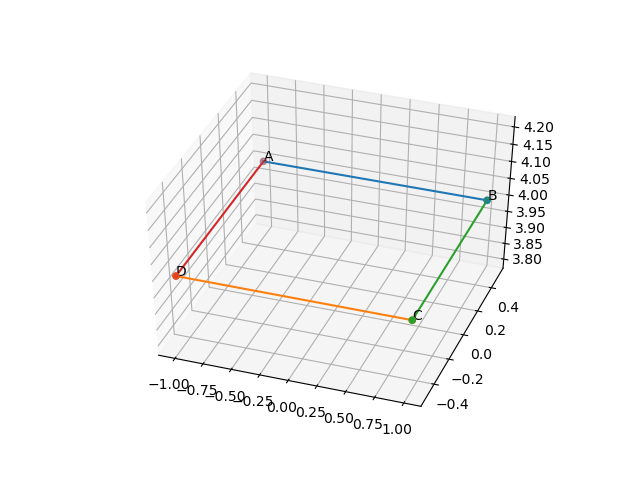
\includegraphics[width=\columnwidth]{chapters/12/10/4/12/figs/Figure_1.png}
   \caption{}
   \label{fig:chapters/12/10/4/12Rect_ABCD}
\end{figure}





\item Find the area of the triangle whose vertices are 
\begin{enumerate}
\item $(2, 3), (–1, 0), (2, – 4)$
\item $(–5, –1), (3, –5), (5, 2)$ 
\end{enumerate}
		\label{10/7/3/1}
\solution
		\iffalse
\documentclass[12pt]{article}
\usepackage{graphicx}
%\documentclass[journal,12pt,twocolumn]{IEEEtran}
\usepackage[none]{hyphenat}
\usepackage{graphicx}
\usepackage{listings}
\usepackage[english]{babel}
\usepackage{graphicx}
\usepackage{caption} 
\usepackage{hyperref}
\usepackage{booktabs}
\usepackage{array}
\usepackage{amsmath}   % for having text in math mode

%Following 2 lines were added to remove the blank page at the beginning
\usepackage{atbegshi}% http://ctan.org/pkg/atbegshi
\AtBeginDocument{\AtBeginShipoutNext{\AtBeginShipoutDiscard}}
%


%New macro definitions
\newcommand{\mydet}[1]{\ensuremath{\begin{vmatrix}#1\end{vmatrix}}}
\providecommand{\brak}[1]{\ensuremath{\left(#1\right)}}
\providecommand{\norm}[1]{\left\lVert#1\right\rVert}
\newcommand{\solution}{\noindent \textbf{Solution: }}
\newcommand{\myvec}[1]{\ensuremath{\begin{pmatrix}#1\end{pmatrix}}}
\let\vec\mathbf

\begin{document}

\begin{center}
\title{\textbf{Area of a Traingle}}
\date{\vspace{-5ex}} %Not to print date automatically
\maketitle
\end{center}

\setcounter{page}{1}



\section{10$^{th}$ Maths - Chapter 7}

This is Problem-1 from Exercise 7.3

\begin{enumerate}
\item Find the area of the triangle whose vertices are :
	\fi
\begin{enumerate}
\item 
In this case, the area  is given by  
  \label{prop:10/7/3/1area2d}
  \begin{align}
    \label{eq:10/7/3/1area2d}
	\frac{1}{2}\norm{\brak{\vec{A}-\vec{B}} \times \brak{\vec{A}-\vec{C}}} \\
  \end{align}
  Since
  \begin{align}
	 \vec{A}-\vec{B} =  \myvec{
  2 \\
  3 \\
 } - \myvec{
  -1 \\
  0 \\
 } = \myvec{
 3 \\
 3 \\
 }
 \\
 \vec{A}-\vec{C} =  \myvec{
  2 \\
  3 \\
 } - \myvec{
  2 \\
  -4 \\
 } = \myvec{
 0 \\
 7 \\
 }
 \end{align}
 the desired area is given by 
 \iffalse
The value of the cross product of two vectors is given by
\begin{align}
  \label{eq:10/7/3/1det2d}
  \mydet{\vec{M}} &= \mydet{\vec{A} & \vec{B}} 
  \\
  &= \mydet{a_1 & b_1\\a_2 & b_2} = a_1b_2 - a_2 b_1
\end{align}

		Therefore, \eqref{eq:10/7/3/1area2d} equals \\
		\fi
\begin{align}
	\frac{1}{2}\mydet{3 & 0\\3 & 7}  
	&=	\frac{21}{2}
\end{align}
\iffalse
\begin{figure}[!h]
	\begin{center}
		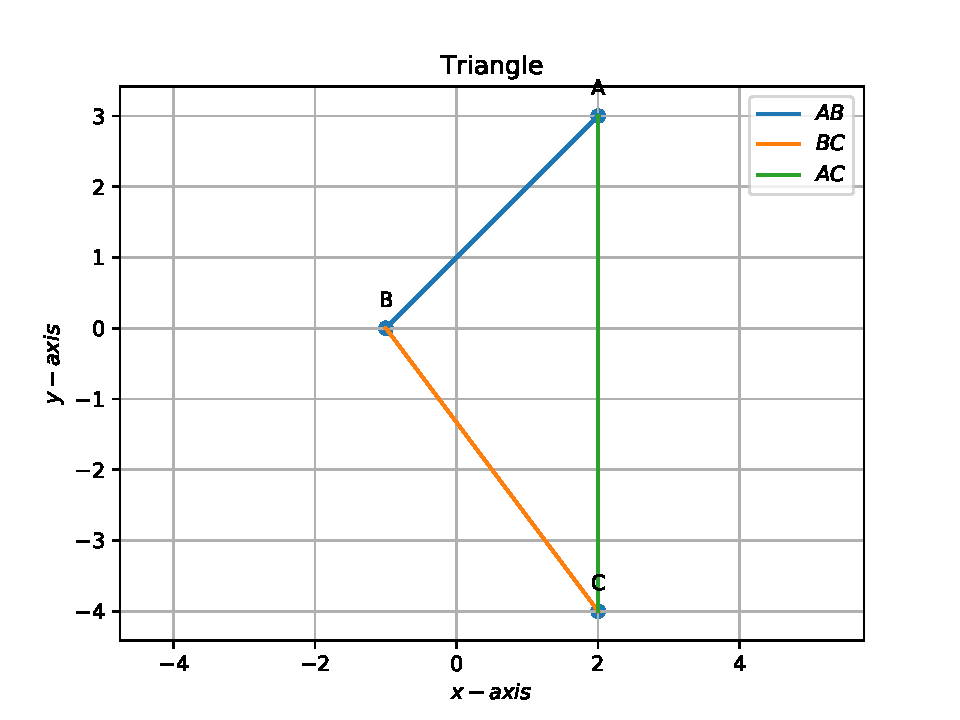
\includegraphics[width=\columnwidth]{./figs/problem1a.pdf}
	\end{center}
\caption{}
\label{fig:Fig1}
\end{figure}
\fi

\item In this case, 
	\iffalse
\solution The area of the triangle with vertices $\vec{A}, \vec{B}, \vec{C}$ is given by  
  \label{prop:10/7/3/1area2e}
  \begin{align}
    \label{eq:10/7/3/1area2e}
	\frac{1}{2}\norm{\brak{\vec{A}-\vec{B}} \times \brak{\vec{A}-\vec{C}}} \\
	\fi
  \begin{align}
	 \vec{A}-\vec{B} =  \myvec{
  -5 \\
  -1 \\
 } - \myvec{
  3 \\
  -5 \\
 } = \myvec{
 -8 \\
 4 \\
 }
 \\
 \vec{A}-\vec{C} =  \myvec{
  -5 \\
  -1 \\
 } - \myvec{
  5 \\
  2 \\
 } = \myvec{
 -10 \\
 -3 \\
 }
 \\
	  \implies
\text{Area} =	\frac{1}{2}\mydet{-8 & -10\\4 & -3}  
	=  32 
\end{align}
\iffalse
\begin{figure}[!h]
	\begin{center}
		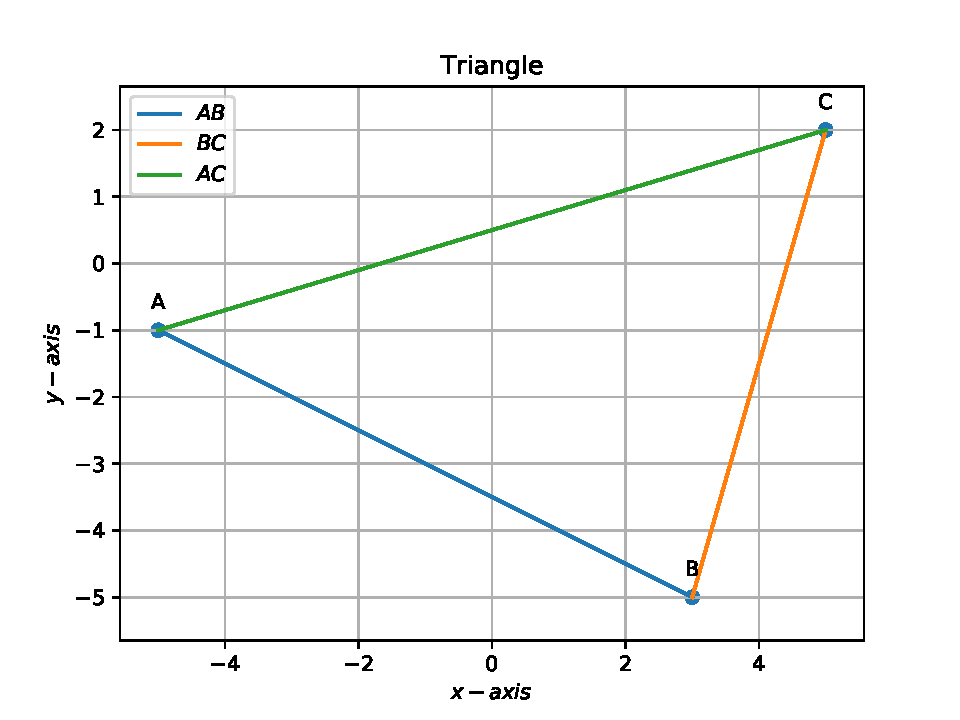
\includegraphics[width=\columnwidth]{./figs/problem1b.pdf}
	\end{center}
\caption{}
\label{fig:Fig2}
\end{figure}
\fi
\end{enumerate}



\item Find the area of the triangle formed by joining the mid-points of the sides of the triangle whose vertices are $(0, –1), (2, 1) \text{ and } (0, 3)$. Find the ratio of this area to the area of the given triangle.
	\\
\solution
		\iffalse
\documentclass[12pt]{article}
\usepackage{graphicx}
\usepackage{amsmath}
\usepackage{mathtools}
\usepackage{gensymb}

\newcommand{\mydet}[1]{\ensuremath{\begin{vmatrix}#1\end{vmatrix}}}
\providecommand{\brak}[1]{\ensuremath{\left(#1\right)}}
\providecommand{\norm}[1]{\left\lVert#1\right\rVert}
\newcommand{\solution}{\noindent \textbf{Solution: }}
\newcommand{\myvec}[1]{\ensuremath{\begin{pmatrix}#1\end{pmatrix}}}
\let\vec\mathbf

\begin{document}
\begin{center}
\textbf\large{CHAPTER-7 \\ COORDINATE GEOMETRY}
\end{center}
\section*{Excercise 7.2}

Q3. Find the area of the triangle formed by joining the mid-points of the sides of the triangle
whose vertices are $\vec(0, –1), \vec(2, 1) \text{ and } \vec(0, 3)$. Find the ratio of this area to the area of the
given triangle
\\
\solution
\\
\fi
The coordinates are given as
	\begin{align}
	\vec{A} = \myvec{
		0\\
		-1\\
		},
	\vec{B} = \myvec{
		2\\
		1\\
		},
	\vec{C} = \myvec{
		0\\
		3\\
		}
	\end{align}
Calculating midpoints,
	\begin{align}
		\vec{P} = \frac{1}{2}\vec(\vec{A}+\vec{B}) = \frac{1}{2}\myvec{2\\0\\} = \myvec{1\\0\\}\\
		\vec{Q} = \frac{1}{2}\vec(\vec{B}+\vec{C}) = \frac{1}{2}\myvec{2\\4\\} = \myvec{1\\2\\}\\
		\vec{R} = \frac{1}{2}\vec(\vec{A}+\vec{C}) = \frac{1}{2}\myvec{0\\2\\} = \myvec{0\\1\\}
	\end{align}
	Since
	\begin{align}
		\vec{P}-\vec{Q} &=  \myvec{
  1 \\
  0 
 } - \myvec{
  1 \\
  2 
 } = \myvec{
 0 \\
 -2 
 }
		\\
		\vec{Q}-\vec{R} &=  \myvec{
  1 \\
  2 \\
 } - \myvec{
  0 \\
  1 \\
 } = \myvec{
 1 \\
 1 \\
 }
	\end{align}
	the area is obtained as
	\begin{align}
		ar(PQR)&=\frac{1}{2}{\norm{\vec(\vec{P}-\vec{Q})\times\vec(\vec{Q}-\vec{R})}}
		\\
		&=\frac{1}{2}\mydet{0 & 1\\-2 & 1}
		=1
	\end{align}
	Similarly, 
	\begin{align}
		\vec{A}-\vec{B} &=  \myvec{
  0 \\
  -1 \\
 } - \myvec{
  2 \\
  1 \\
 } = \myvec{
 -2 \\
 -2 \\
 }
 \\
		\vec{A}-\vec{C} &=  \myvec{
  0 \\
  -1 \\
 } - \myvec{
  0 \\
  3 \\
 } = \myvec{
 0 \\
 -4 \\
 }
	\end{align}
 the area is obained as
	\begin{align}
		ar(ABC)&=\frac{1}{2}{\norm{\vec(\vec{A}-\vec{B})\times\vec(\vec{A}-\vec{C})}}\\
		&=\frac{1}{2}\mydet{-2 & 0\\-2 & -4}
=4
	\end{align}
	Thus, the resultant ratio of two areas is 1:4.
	See Fig.
\ref{fig:10/7/3/3Fig}
\begin{figure}[!h]
	\begin{center} 
	    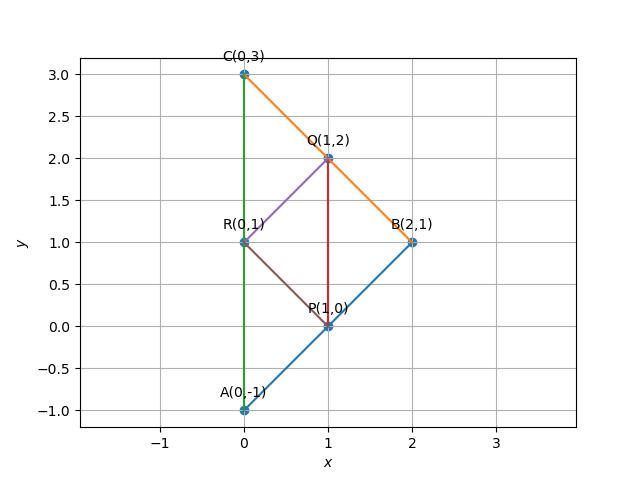
\includegraphics[width=\columnwidth]{chapters/10/7/3/3/figs/trigraph.png}
	\end{center}
\caption{}
\label{fig:10/7/3/3Fig}
\end{figure}


\item Find the area of the quadrilateral whose vertices, taken in order, are $(– 4, – 2), (– 3, – 5), (3, – 2)$  and $ (2, 3)$.
	\\
\solution
		\iffalse
\documentclass[12pt]{article}
\usepackage{graphicx}
%\documentclass[journal,12pt,twocolumn]{IEEEtran}
\usepackage[none]{hyphenat}
\usepackage{graphicx}
\usepackage{listings}
\usepackage[english]{babel}
\usepackage{graphicx}
\usepackage{caption} 
\usepackage{hyperref}
\usepackage{booktabs}
\def\inputGnumericTable{}
\usepackage{color}                                            %%
    \usepackage{array}                                            %%
    \usepackage{longtable}                                        %%
    \usepackage{calc}                                             %%
    \usepackage{multirow}                                         %%
    \usepackage{hhline}                                           %%
    \usepackage{ifthen}
\usepackage{array}
\usepackage{amsmath}   % for having text in math mode
\usepackage{listings}
\lstset{
language=tex,
frame=single, 
breaklines=true
}
  
%Following 2 lines were added to remove the blank page at the beginning
\usepackage{atbegshi}% http://ctan.org/pkg/atbegshi
\AtBeginDocument{\AtBeginShipoutNext{\AtBeginShipoutDiscard}}
%
%New macro definitions
\newcommand{\mydet}[1]{\ensuremath{\begin{vmatrix}#1\end{vmatrix}}}
\providecommand{\brak}[1]{\ensuremath{\left(#1\right)}}
\providecommand{\norm}[1]{\left\lVert#1\right\rVert}
\newcommand{\solution}{\noindent \textbf{Solution: }}
\newcommand{\myvec}[1]{\ensuremath{\begin{pmatrix}#1\end{pmatrix}}}
\let\vec\mathbf
\begin{document}
\begin{center}
\title{\textbf{Coordinate Geometry}}
\date{\vspace{-5ex}} %Not to print date automatically
\maketitle
\end{center}
\setcounter{page}{1}
\section*{10$^{th}$ Maths - Chapter 7}
This is Problem-4 from Exercise 7.3
\begin{enumerate}
\item Find the area of quadrilateral whose vertices, taken in order, are $\myvec{-4 \\ -2}, \myvec{-3\\-5}, \myvec{3\\-2}$ and $\myvec{2\\3}$.\\
	\solution 
\fi
		The input parameters for this problem are available in Table \eqref{tab:10/7/3/4}.
\begin{table}[ht!]\centering
%%%%%%%%%%%%%%%%%%%%%%%%%%%%%%%%%%%%%%%%%%%%%%%%%%%%%%%%%%%%%%%%%%%%%%
%%                                                                  %%
%%  This is the header of a LaTeX2e file exported from Gnumeric.    %%
%%                                                                  %%
%%  This file can be compiled as it stands or included in another   %%
%%  LaTeX document. The table is based on the longtable package so  %%
%%  the longtable options (headers, footers...) can be set in the   %%
%%  preamble section below (see PRAMBLE).                           %%
%%                                                                  %%
%%  To include the file in another, the following two lines must be %%
%%  in the including file:                                          %%
%%        \def\inputGnumericTable{}                                 %%
%%  at the beginning of the file and:                               %%
%%        \input{name-of-this-file.tex}                             %%
%%  where the table is to be placed. Note also that the including   %%
%%  file must use the following packages for the table to be        %%
%%  rendered correctly:                                             %%
%%    \usepackage[latin1]{inputenc}                                 %%
%%    \usepackage{color}                                            %%
%%    \usepackage{array}                                            %%
%%    \usepackage{longtable}                                        %%
%%    \usepackage{calc}                                             %%
%%    \usepackage{multirow}                                         %%
%%    \usepackage{hhline}                                           %%
%%    \usepackage{ifthen}                                           %%
%%  optionally (for landscape tables embedded in another document): %%
%%    \usepackage{lscape}                                           %%
%%                                                                  %%
%%%%%%%%%%%%%%%%%%%%%%%%%%%%%%%%%%%%%%%%%%%%%%%%%%%%%%%%%%%%%%%%%%%%%%



%%  This section checks if we are begin input into another file or  %%
%%  the file will be compiled alone. First use a macro taken from   %%
%%  the TeXbook ex 7.7 (suggestion of Han-Wen Nienhuys).            %%
\def\ifundefined#1{\expandafter\ifx\csname#1\endcsname\relax}


%%  Check for the \def token for inputed files. If it is not        %%
%%  defined, the file will be processed as a standalone and the     %%
%%  preamble will be used.                                          %%
\ifundefined{inputGnumericTable}

%%  We must be able to close or not the document at the end.        %%
 \def\gnumericTableEnd{\end{document}}


%%%%%%%%%%%%%%%%%%%%%%%%%%%%%%%%%%%%%%%%%%%%%%%%%%%%%%%%%%%%%%%%%%%%%%
%%                                                                  %%
%%  This is the PREAMBLE. Change these values to get the right      %%
%%  paper size and other niceties.                                  %%
%%                                                                  %%
%%%%%%%%%%%%%%%%%%%%%%%%%%%%%%%%%%%%%%%%%%%%%%%%%%%%%%%%%%%%%%%%%%%%%%

 \documentclass[12pt%
     %,landscape%
                    ]{report}
       \usepackage[latin1]{inputenc}
       \usepackage{fullpage}
       \usepackage{color}
       \usepackage{array}
       \usepackage{longtable}
       \usepackage{calc}
       \usepackage{multirow}
       \usepackage{hhline}
       \usepackage{ifthen}

 \begin{document}


%%  End of the preamble for the standalone. The next section is for %%
%%  documents which are included into other LaTeX2e files.          %%
\else

%%  We are not a stand alone document. For a regular table, we will %%
%%  have no preamble and only define the closing to mean nothing.   %%
    \def\gnumericTableEnd{}

%%  If we want landscape mode in an embedded document, comment out  %%
%%  the line above and uncomment the two below. The table will      %%
%%  begin on a new page and run in landscape mode.                  %%
%       \def\gnumericTableEnd{\end{landscape}}
%       \begin{landscape}


%%  End  theoelse clause for this file being \input.              %%
\fi

%%%%%%%%%%%%%%%%%%%%%%%%%%%%%%%%%%%%%%%%%%%%%%%%%%%%%%%%%%%%%%%%%%%%%%
%%                                                                  %%
%%  The rest is the gnumeric table, except for the closing          %%
%%  statement. Changes below will alter the table's appearance.     %%
%%                                                                  %%
%%%%%%%%%%%%%%%%%%%%%%%%%%%%%%%%%%%%%%%%%%%%%%%%%%%%%%%%%%%%%%%%%%%%%%

\providecommand{\gnumericmathit}[1]{#1} 
%%  Uncomment the next line if you would like your numbers to be in %%
%%  italics if they are italizised in the gnumeric table.           %%
%\renewcommand{\gnumericmathit}[1]{\mathit{#1}}
\providecommand{\gnumericPB}[1]%
{\let\gnumericTemp=\\#1\let\\=\gnumericTemp\hspace{0pt}}
 \ifundefined{gnumericTableWidthDefined}
        \newlength{\gnumericTableWidth}
        \newlength{\gnumericTableWidthComplete}
        \newlength{\gnumericMultiRowLength}
        \global\def\gnumericTableWidthDefined{}
 \fi
%% The following setting protects this code from babel shorthands.  %%
 \ifthenelse{\isundefined{\languageshorthands}}{}{\languageshorthands{english}}
%%  The default table format retains the relative column widths of  %%
%%  gnumeric. They can easily be changed to c, r or l. In that case %%
%%  you may want to comment out the next line and uncomment the one %%
%%  thereafter                                                      %%
\providecommand\gnumbox{\makebox[0pt]}
%%\providecommand\gnumbox[1][]{\makebox}

%% to adjust positions in multirow situations                       %%
\setlength{\bigstrutjot}{\jot}
\setlength{\extrarowheight}{\doublerulesep}

%%  The \setlongtables command keeps column widths the same across  %%
%%  pages. Simply comment out next line for varying column widths.  %%
\setlongtables

\setlength\gnumericTableWidth{%
 53pt+%
 53pt+%
 82pt+%
 53pt+%
0pt}
\def\gumericNumCols{4}
\setlength\gnumericTableWidthComplete{\gnumericTableWidth+%
         \tabcolsep*\gumericNumCols*2+\arrayrulewidth*\gumericNumCols}
\ifthenelse{\lengthtest{\gnumericTableWidthComplete > \linewidth}}%
         {\def\gnumericScale{1*\ratio{\linewidth-%
                        \tabcolsep*\gumericNumCols*2-%
                        \arrayrulewidth*\gumericNumCols}%
{\gnumericTableWidth}}}%
{\def\gnumericScale{1}}

%%%%%%%%%%%%%%%%%%%%%%%%%%%%%%%%%%%%%%%%%%%%%%%%%%%%%%%%%%%%%%%%%%%%%%
%%                                                                  %%
%% The following are the widths of the various columns. We are      %%
%% defining them here because then they are easier to change.       %%
%% Depending on the cell formats we may use them more than once.    %%
%%                                                                  %%
%%%%%%%%%%%%%%%%%%%%%%%%%%%%%%%%%%%%%%%%%%%%%%%%%%%%%%%%%%%%%%%%%%%%%%

\ifthenelse{\isundefined{\gnumericColA}}{\newlength{\gnumericColA}}{}\settowidth{\gnumericColA}{\begin{tabular}{@{}p{53pt*\gnumericScale}@{}}x\end{tabular}}
\ifthenelse{\isundefined{\gnumericColB}}{\newlength{\gnumericColB}}{}\settowidth{\gnumericColB}{\begin{tabular}{@{}p{53pt*\gnumericScale}@{}}x\end{tabular}}
\ifthenelse{\isundefined{\gnumericColC}}{\newlength{\gnumericColC}}{}\settowidth{\gnumericColC}{\begin{tabular}{@{}p{82pt*\gnumericScale}@{}}x\end{tabular}}
\ifthenelse{\isundefined{\gnumericColD}}{\newlength{\gnumericColD}}{}\settowidth{\gnumericColD}{\begin{tabular}{@{}p{53pt*\gnumericScale}@{}}x\end{tabular}}

\begin{center}
\begin{tabular}[c]{%
 b{\gnumericColA}%
 b{\gnumericColB}%
 b{\gnumericColC}%
 b{\gnumericColD}%
 }

%%%%%%%%%%%%%%%%%%%%%%%%%%%%%%%%%%%%%%%%%%%%%%%%%%%%%%%%%%%%%%%%%%%%%%
%%  The longtable options. (Caption, headers... see Goosens, p.124) %%
% \caption{The Table Caption.}             \\ %
% \hline % Across the top of the table.
%%  The rest of these options are table rows which are placed on    %%
%%  the first, last or every page. Use \multicolumn if you want.    %%

%%  Header for the first page.                                      %%
% \multicolumn{4}{c}{The First Header} \\ \hline 
% \multicolumn{1}{c}{colTag} %Column 1
% &\multicolumn{1}{c}{colTag} %Column 2
% &\multicolumn{1}{c}{colTag} %Column 3
% &\multicolumn{1}{c}{colTag} \\ \hline %Last column
% \endfirsthead

%%  The running header definition.                                  %%
% \hline
% \multicolumn{4}{l}{\ldots\small\slshape continued} \\ \hline
% \multicolumn{1}{c}{colTag} %Column 1
% &\multicolumn{1}{c}{colTag} %Column 2
% &\multicolumn{1}{c}{colTag} %Column 3
% &\multicolumn{1}{c}{colTag} \\ \hline %Last column
% \endhead

%%  The running footer definition.                                  %%
% \hline
% \multicolumn{4}{r}{\small\slshape continued\ldots} \\
% \endfoot

%%  The ending footer definition.                                   %%
% \multicolumn{4}{c}{That's all folks} \\ \hline 
% \endlastfoot
%%%%%%%%%%%%%%%%%%%%%%%%%%%%%%%%%%%%%%%%%%%%%%%%%%%%%%%%%%%%%%%%%%%%%%

\hhline{|-|-|-~}
  \multicolumn{1}{|p{\gnumericColA}|}%
 {\gnumericPB{\centering}\gnumbox{\textbf{Symbol}}}
 &\multicolumn{1}{p{\gnumericColB}|}%
 {\gnumericPB{\centering}\gnumbox{\textbf{Value}}}
 &\multicolumn{1}{p{\gnumericColC}|}%
 {\gnumericPB{\centering}\gnumbox{\textbf{Description}}}
 &
\\
\hhline{|---|~}
  \multicolumn{1}{|p{\gnumericColA}|}%
 {\gnumericPB{\centering}\gnumbox{$\vec{A}$}}
 &\multicolumn{1}{p{\gnumericColB}|}%
 {\gnumericPB{\centering}\gnumbox{$\myvec{-4\\-2}$}}
 &\multicolumn{1}{p{\gnumericColC}|}%
 {\gnumericPB{\centering}\gnumbox{First point}}
 &
\\
\hhline{|---|~}
  \multicolumn{1}{|p{\gnumericColA}|}%
 {\gnumericPB{\centering}\gnumbox{$\vec{B}$}}
 &\multicolumn{1}{p{\gnumericColB}|}%
 {\gnumericPB{\centering}\gnumbox{$\myvec{-3\\-5}$}}
 &\multicolumn{1}{p{\gnumericColC}|}%
 {\gnumericPB{\centering}\gnumbox{Second point}}
 &
\\
\hhline{|---|~}
  \multicolumn{1}{|p{\gnumericColA}|}%
 {\gnumericPB{\centering}\gnumbox{$\vec{C}$}}
 &\multicolumn{1}{p{\gnumericColB}|}%
 {\gnumericPB{\centering}\gnumbox{$\myvec{3\\-2}$}}
 &\multicolumn{1}{p{\gnumericColC}|}%
 {\gnumericPB{\centering}\gnumbox{Third point}}
 &
\\

\hhline{|---|~}
  \multicolumn{1}{|p{\gnumericColA}|}%
 {\gnumericPB{\centering}\gnumbox{$\vec{D}$}}
 &\multicolumn{1}{p{\gnumericColB}|}%
 {\gnumericPB{\centering}\gnumbox{$\myvec{2\\3}$}}
 &\multicolumn{1}{p{\gnumericColC}|}%
 {\gnumericPB{\centering}\gnumbox{Fourth point}}
 &
\\
\hhline{|-|-|-|~}
\end{tabular}
 \end{center}

\ifthenelse{\isundefined{\languageshorthands}}{}{\languageshorthands{\languagename}}
%\gnumericTableEndf

\caption{}
\label{tab:10/7/3/4}	
\end{table}
By joining $\vec{B}$ to $\vec{D}$, two triangles $\vec{A}\vec{B}\vec{D}$ and $\vec{B}\vec{C}\vec{D}$ are obtained.
Since
\begin{align}
	\vec{A}- \vec{B} &= \myvec{-4\\-2\\}-\myvec{-3\\-5\\}=\myvec{-1\\3\\}\label{eq:chapters/10/7/3/4/2}\\
	  \vec{A}- \vec{D} &= \myvec{-4\\-2\\}-\myvec{2\\3\\}=\myvec{-6\\-5\\}\label{eq:chapters/10/7/3/4/3}
  \end{align}
  \begin{align}
	  ar(ABD)&=\frac{1}{2} \norm{\brak{\vec{A}-\vec{B}}  \times 
   \brak{\vec{A}- \vec{D}}} \label{eq:chapters/10/7/3/4/1} 
   \\
	  &=	\frac{1}{2}\mydet{-1 & 3\\-6 & -5}  
	=	\frac{23}{2}
\end{align}
upon substituting the values of \eqref{eq:chapters/10/7/3/4/2} and \eqref{eq:chapters/10/7/3/4/3} in \eqref{eq:chapters/10/7/3/4/1}.
Similarly,
\begin{align}
	\vec{B}- \vec{C} &= \myvec{-3\\-5\\}-\myvec{3\\-2\\}=\myvec{-6\\-5\\}\label{eq:chapters/10/7/3/4/6} \\
	  \vec{B}- \vec{D} &= \myvec{-3\\-5\\}-\myvec{2\\3\\}=\myvec{-3\\-8\\}\label{eq:chapters/10/7/3/4/7} 
  \end{align}
  yielding
  \begin{align}
	  ar(BCD)&=\frac{1}{2} \norm{\brak{\vec{B}-\vec{C}}  \times 
   \brak{\vec{B}- \vec{D}}} \label{eq:chapters/10/7/3/4/5}
   \\
	  &=	\frac{1}{2}\mydet{-6 & -3\\-5 & -8}  
	=	\frac{33}{2}
\end{align}
	upon 	substituting the values of \eqref{eq:chapters/10/7/3/4/6} and \eqref{eq:chapters/10/7/3/4/7} in \eqref{eq:chapters/10/7/3/4/5}
		Thus, 
\begin{align}
	ar(ABCD)&=  ar(ABD) +  ar(BCD)
	= 28
\end{align}
See Fig. 
\ref{fig:chapters/10/7/3/4/Fig1}
\begin{figure}[!h]
 \begin{center}
  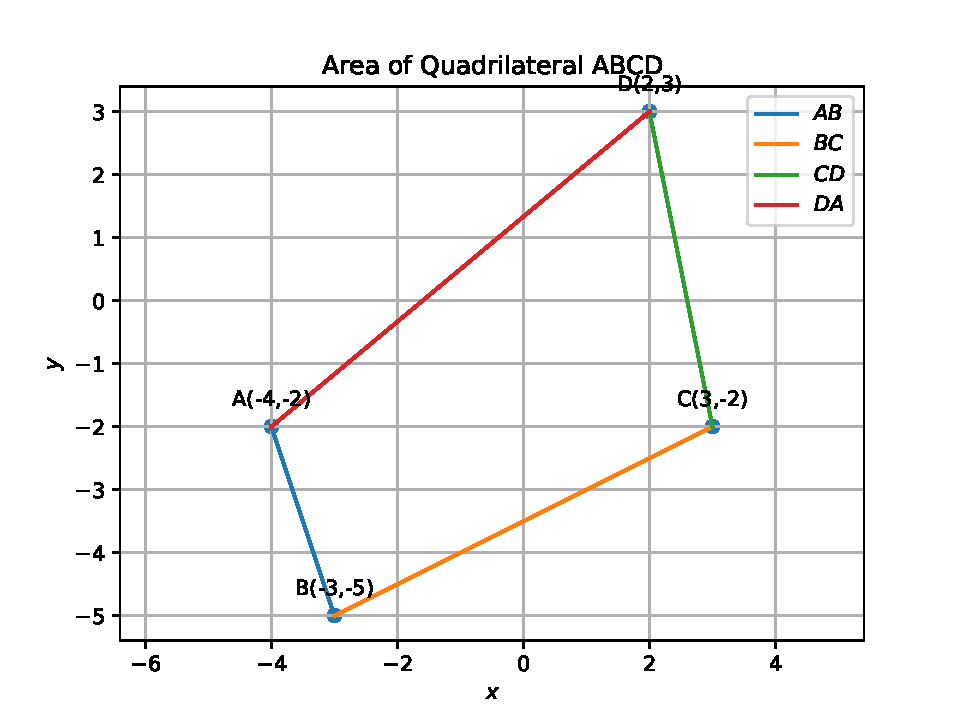
\includegraphics[width=\columnwidth]{chapters/10/7/3/4/figs/fig.pdf}
 \end{center}
\caption{}
\label{fig:chapters/10/7/3/4/Fig1}
\end{figure}


\item Verify that a median of a triangle divides it into two triangles of equal areas for $\triangle ABC$ whose vertices are $\vec{A}(4, -6), \vec{B}(3, 2), \text{ and } \vec{C}(5, 2)$. 
		\label{10/7/3/5}
		\\
\solution
		\iffalse
\documentclass[12pt]{article}
\usepackage{graphicx}
\usepackage[none]{hyphenat}
\usepackage{graphicx}
\usepackage{listings}
\usepackage[english]{babel}
\usepackage{graphicx}
\usepackage{caption} 
\usepackage{booktabs}
\usepackage{array}
\usepackage{amssymb} % for \because
\usepackage{amsmath}   % for having text in math mode
\usepackage{extarrows} % for Row operations arrows
\usepackage{listings}
\usepackage[utf8]{inputenc}
\lstset{
  frame=single,
  breaklines=true
}
\usepackage{hyperref}
  
%Following 2 lines were added to remove the blank page at the beginning
\usepackage{atbegshi}% http://ctan.org/pkg/atbegshi
\AtBeginDocument{\AtBeginShipoutNext{\AtBeginShipoutDiscard}}


%New macro definitions
\newcommand{\mydet}[1]{\ensuremath{\begin{vmatrix}#1\end{vmatrix}}}
\providecommand{\brak}[1]{\ensuremath{\left(#1\right)}}
\newcommand{\solution}{\noindent \textbf{Solution: }}
\newcommand{\myvec}[1]{\ensuremath{\begin{pmatrix}#1\end{pmatrix}}}
\providecommand{\norm}[1]{\left\lVert#1\right\rVert}
\providecommand{\abs}[1]{\left\vert#1\right\vert}
\let\vec\mathbf

\begin{document}

\begin{center}
\title{\textbf{VECTORS}}
\date{\vspace{-5ex}} %Not to print date automatically
\maketitle
\end{center}

\section{10$^{th}$ Maths - EXERCISE-7.3}

\begin{enumerate}
\item That a median of a triangle divides it into two triangles  of equal areas. verify this result for $\triangle ABC$ whose vertices are $\vec{A}(4,-6),\vec{B}(3,-2)\text{ and }\vec{C}(5,2)$.
\end{enumerate}

\section{SOLUTION}
Given points are
\begin{align}
\vec{A}=\myvec{4\\ -6} ,
\vec{B}=\myvec{3\\ -2} ,
\vec{C}=\myvec{5\\ 2}
\end{align}
\fi
The median of the triangle 
\begin{align}
\vec{D}&=\frac{\vec{B}+\vec{C}}{2}\\
&=\myvec{4\\ 0}
\end{align}
Since 
\begin{align}
	\vec{A}- \vec{B} &= \myvec{4\\ -6}-\myvec{3\\ -2}=\myvec{1\\ -4}\label{eq:10/7/3/5/7}\\
	  \vec{A}- \vec{D} &= \myvec{4\\ -6}-\myvec{4\\ 0}=\myvec{0\\ -6}\label{eq:10/7/3/5/8}
  \end{align}
 \begin{align}
  ar(ABD)&=\frac{1}{2} \norm{\brak{\vec{A}-\vec{B}}  \times 
   \brak{\vec{A}- \vec{D}}} \label{eq:10/7/3/5/6} 
   \\
&=\frac{1}{2}\mydet{1 & 0\\-4 & -6}
	       =3	
\end{align}
upon
Substituting from \eqref{eq:10/7/3/5/7} and \eqref{eq:10/7/3/5/8} in \eqref{eq:10/7/3/5/6}.
		Similarly, 
\begin{align}
	\vec{A}- \vec{C} &= \myvec{4\\ -6}-\myvec{5\\ 2}=\myvec{-1\\ -8}\label{eq:10/7/3/5/13} \\
	  \vec{A}- \vec{D} &= \myvec{4\\ -6}-\myvec{4\\ 0}=\myvec{0\\ -6}\label{eq:10/7/3/5/14} 
  \end{align}
  yielding
  \begin{align}
  ar(ACD)&=\frac{1}{2} \norm{\brak{\vec{A}-\vec{C}}  \times 
   \brak{\vec{A}- \vec{D}}} \label{eq:10/7/3/5/12}
   \\
	&=\frac{1}{2}\mydet{-1 & 0\\-8 & -6}= 3
\end{align}
upon substituting from \eqref{eq:10/7/3/5/13} and \eqref{eq:10/7/3/5/14} in \eqref{eq:10/7/3/5/12}.
Thus,
\begin{align}
ar(ABD)=ar(ACD)
\end{align}
See Fig. 
\ref{fig:10/7/3/5/}.
\begin{figure}[h!]
\centering
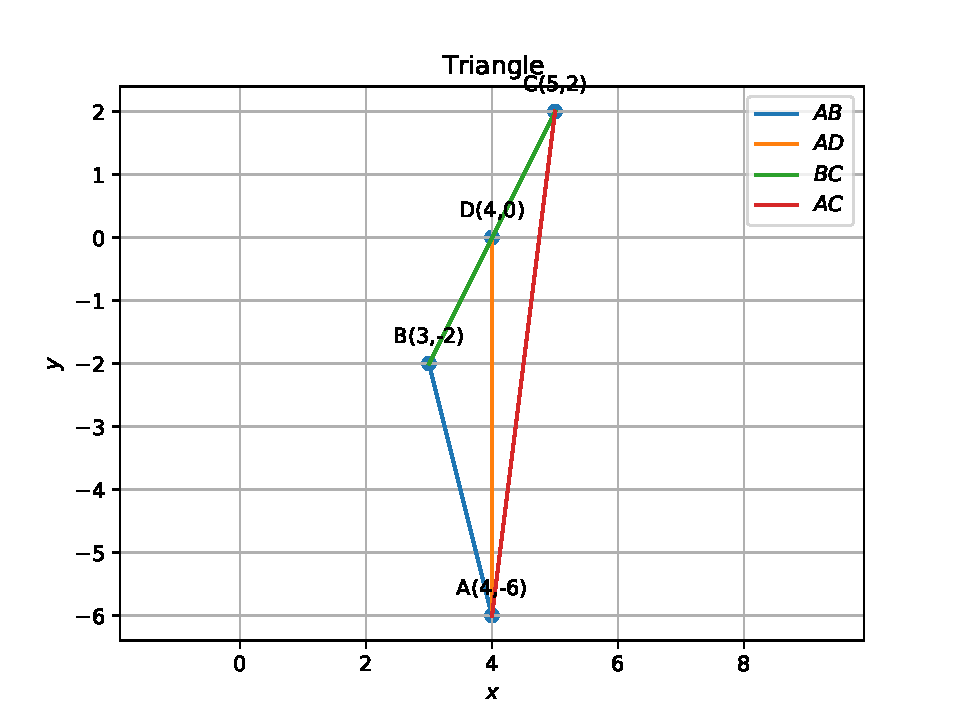
\includegraphics[width=\columnwidth]{chapters/10/7/3/5/figs/fig.pdf}
\caption{}
\label{fig:10/7/3/5/}
\end{figure} 


\item The two adjacent sides of a parallelogram are 
$2\hat{i}-4\hat{j}+5\hat{k}$  and  $\hat{i}-2\hat{j}-3\hat{k}$.
Find the unit vector parallel to its diagonal. Also, find its area.\\
	\solution
		\iffalse
\documentclass[journal,12pt,twocolumn]{IEEEtran}
\usepackage{setspace}
\usepackage{gensymb}
\usepackage{xcolor}
\usepackage{caption}
\singlespacing
\usepackage{siunitx}
\usepackage[cmex10]{amsmath}
\usepackage{mathtools}
\usepackage{hyperref}
\usepackage{amsthm}
\usepackage{mathrsfs}
\usepackage{txfonts}
\usepackage{stfloats}
\usepackage{cite}
\usepackage{cases}
\usepackage{subfig}
\usepackage{longtable}
\usepackage{multirow}
\usepackage{enumitem}
\usepackage{bm}
\usepackage{mathtools}
\usepackage{listings}
\usepackage{tikz}
\usetikzlibrary{shapes,arrows,positioning}
\usepackage{circuitikz}
\renewcommand{\vec}[1]{\boldsymbol{\mathbf{#1}}}
\DeclareMathOperator*{\Res}{Res}
\renewcommand\thesection{\arabic{section}}
\renewcommand\thesubsection{\thesection.\arabic{subsection}}
\renewcommand\thesubsubsection{\thesubsection.\arabic{subsubsection}}

\renewcommand\thesectiondis{\arabic{section}}
\renewcommand\thesubsectiondis{\thesectiondis.\arabic{subsection}}
\renewcommand\thesubsubsectiondis{\thesubsectiondis.\arabic{subsubsection}}
\hyphenation{op-tical net-works semi-conduc-tor}

\lstset{
language=Python,
frame=single, 
breaklines=true,
columns=fullflexible
}
\begin{document}
\theoremstyle{definition}
\newtheorem{theorem}{Theorem}[section]
\newtheorem{problem}{Problem}
\newtheorem{proposition}{Proposition}[section]
\newtheorem{lemma}{Lemma}[section]
\newtheorem{corollary}[theorem]{Corollary}
\newtheorem{example}{Example}[section]
\newtheorem{definition}{Definition}[section]
\newcommand{\BEQA}{\begin{eqnarray}}
        \newcommand{\EEQA}{\end{eqnarray}}
\newcommand{\define}{\stackrel{\triangle}{=}}
\newcommand{\myvec}[1]{\ensuremath{\begin{pmatrix}#1\end{pmatrix}}}
\newcommand{\mydet}[1]{\ensuremath{\begin{vmatrix}#1\end{vmatrix}}}
\bibliographystyle{IEEEtran}
\providecommand{\nCr}[2]{\,^{#1}C_{#2}} % nCr
\providecommand{\nPr}[2]{\,^{#1}P_{#2}} % nPr
\providecommand{\mbf}{\mathbf}
\providecommand{\pr}[1]{\ensuremath{\Pr\left(#1\right)}}
\providecommand{\qfunc}[1]{\ensuremath{Q\left(#1\right)}}
\providecommand{\sbrak}[1]{\ensuremath{{}\left[#1\right]}}
\providecommand{\lsbrak}[1]{\ensuremath{{}\left[#1\right.}}
\providecommand{\rsbrak}[1]{\ensuremath{{}\left.#1\right]}}
\providecommand{\brak}[1]{\ensuremath{\left(#1\right)}}
\providecommand{\lbrak}[1]{\ensuremath{\left(#1\right.}}
\providecommand{\rbrak}[1]{\ensuremath{\left.#1\right)}}
\providecommand{\cbrak}[1]{\ensuremath{\left\{#1\right\}}}
\providecommand{\lcbrak}[1]{\ensuremath{\left\{#1\right.}}
\providecommand{\rcbrak}[1]{\ensuremath{\left.#1\right\}}}
\theoremstyle{remark}
\newtheorem{rem}{Remark}
\newcommand{\sgn}{\mathop{\mathrm{sgn}}}
\newcommand{\rect}{\mathop{\mathrm{rect}}}
\newcommand{\sinc}{\mathop{\mathrm{sinc}}}
\providecommand{\abs}[1]{\left\vert#1\right\vert}
\providecommand{\res}[1]{\Res\displaylimits_{#1}}
\providecommand{\norm}[1]{\lVert#1\rVert}
\providecommand{\mtx}[1]{\mathbf{#1}}
\providecommand{\mean}[1]{E\left[ #1 \right]}
\providecommand{\fourier}{\overset{\mathcal{F}}{ \rightleftharpoons}}
\providecommand{\ztrans}{\overset{\mathcal{Z}}{ \rightleftharpoons}}
\providecommand{\system}[1]{\overset{\mathcal{#1}}{ \longleftrightarrow}}
\newcommand{\solution}{\noindent \textbf{Solution: }}
\providecommand{\dec}[2]{\ensuremath{\overset{#1}{\underset{#2}{\gtrless}}}}
\let\StandardTheFigure\thefigure
\def\putbox#1#2#3{\makebox[0in][l]{\makebox[#1][l]{}\raisebox{\baselineskip}[0in][0in]{\raisebox{#2}[0in][0in]{#3}}}}
\def\rightbox#1{\makebox[0in][r]{#1}}
\def\centbox#1{\makebox[0in]{#1}}
\def\topbox#1{\raisebox{-\baselineskip}[0in][0in]{#1}}
\def\midbox#1{\raisebox{-0.5\baselineskip}[0in][0in]{#1}}

\vspace{3cm}
\title{12.10.5.10}
\author{Lokesh Surana}
\maketitle
\section*{Class 12, Chapter 10, Exercise 5.10}

Q.10. The two adjacent sides of a parallelogram are  ${2}\hat{i} -  {4}\hat{j} + {5}\hat{k}$ and ${1}\hat{i} -  {2}\hat{j} - {3}\hat{k}$.
Find the unit vector parallel to its diagonal. Also, find its area.

\solution 
\fi
Let the sides of the parallelogram be 
\begin{align}
\vec{a} = \myvec{2\\-4\\5}, \, \vec{b} = \myvec{1\\-2\\-3}.
\end{align}
The diagonals of the parallelogram are given by
\begin{align}
	\vec{D}_1 &= \vec{a} + \vec{b} = \myvec{3 \\-6\\2} \\
	\vec{D}_2 &= \vec{a} - \vec{b} = \myvec{1 \\-2\\8}
\end{align}
The unit vectors parallel to the diagonals are then given by
\begin{align}
	\hat{\vec{D}_1} &= \frac{\vec{D}_1}{\norm{\vec{D}_1}}  = \myvec{\frac{3}{\sqrt{45}}\\-\frac{6}{\sqrt{45}}\\\frac{2}{\sqrt{45}}} \\
    \hat{\vec{D}_2} &= \frac{\vec{D}_2}{\norm{\vec{D}_2}}  = \myvec{\frac{1}{\sqrt{69}}\\-\frac{2}{\sqrt{69}}\\\frac{8}{\sqrt{69}}}
\end{align}
%
Since
\begin{align}
    \vec{a}\times\vec{b}=\myvec{22 \\-11\\0},
\end{align}
he area of the parallelogram is given by
\begin{align}
    \norm{\vec{a}\times\vec{b}}  = \sqrt{605}
\end{align}


\item The vertices of a $\triangle ABC$ are $\vec{A}(4,6), \vec{B}(1,5)$ and  $\vec{C}(7,2)$. A line is drawn to intersect sides $AB$ and $AC$ at $\vec{D}$ and $\vec{E}$ respectively, such that $\frac{AD}{AB} = \frac{AE}{AC} = \frac{1}{4}$. Calculate the area of $\triangle ADE$ and compare it with the area of the $\triangle ABC$.
\\
\solution
	\iffalse
\documentclass[12pt]{article}
\usepackage{graphicx}
%\documentclass[journal,12pt,twocolumn]{IEEEtran}
\usepackage[none]{hyphenat}
\usepackage{graphicx}
\usepackage{listings}
\usepackage[english]{babel}
\usepackage{graphicx}
\usepackage{caption}
\usepackage[parfill]{parskip}
\usepackage{hyperref}
\usepackage{booktabs}
%\usepackage{setspace}\doublespacing\pagestyle{plain}
\def\inputGnumericable{}
\usepackage{color}                                            %%
    \usepackage{array}                                            %%
    \usepackage{longtable}                                        %%
    \usepackage{calc}                                             %%
    \usepackage{multirow}                                         %%
    \usepackage{hhline}                                           %%
    \usepackage{ifthen}
\usepackage{array}
\usepackage{amsmath}   % for having text in math mode
\usepackage{parallel,enumitem}
\usepackage{listings}
\lstset{
language=tex,
frame=single, 
breaklines=true
}
  
%Following 2 lines were added to remove the blank page at the beginning
\usepackage{atbegshi}% http://ctan.org/pkg/atbegshi
\AtBeginDocument{\AtBeginShipoutNext{\AtBeginShipoutDiscard}}
%
%New macro definitions
\newcommand{\mydet}[1]{\ensuremath{\begin{vmatrix}#1\end{vmatrix}}}
\providecommand{\brak}[1]{\ensuremath{\left(#1\right)}}
\providecommand{\norm}[1]{\left\lVert#1\right\rVert}
\newcommand{\solution}{\noindent \textbf{Solution: }}
\newcommand{\myvec}[1]{\ensuremath{\begin{pmatrix}#1\end{pmatrix}}}
\let\vec\mathbf
\begin{document}
\begin{center}
\title{\textbf{Coordinate Geometry}}
\date{\vspace{-5ex}} %Not to print date automatically
\maketitle
\end{center}
\setcounter{page}{1}
\section*{10$^{th}$ Maths - Chapter 7}
This is Problem-6 from Exercise 7.4
\begin{enumerate}
\item The vertices of $\triangle ABC$ are $\myvec{4 \\ 6}, \myvec{1\\5}, \myvec{7\\2}$. A line is drawn to intersect sides AB and AC at D and E respectively, such that $\dfrac{AD}{AB}=\dfrac{AE}{AC}=\dfrac{1}{4}$. Calculate the area of the $\triangle ADE$ and compare it with the area of $\triangle ABC$.\\
\solution 
\fi
		The input parameters for this problem are available in Table \eqref{table:chapters/10/7/4/61}.
\begin{table}[ht!]\centering
%%%%%%%%%%%%%%%%%%%%%%%%%%%%%%%%%%%%%%%%%%%%%%%%%%%%%%%%%%%%%%%%%%%%%%
%%                                                                  %%
%%  This is the header of a LaTeX2e file exported from Gnumeric.    %%
%%                                                                  %%
%%  This file can be compiled as it stands or included in another   %%
%%  LaTeX document. The table is based on the longtable package so  %%
%%  the longtable options (headers, footers...) can be set in the   %%
%%  preamble section below (see PRAMBLE).                           %%
%%                                                                  %%
%%  To include the file in another, the following two lines must be %%
%%  in the including file:                                          %%
%%        \def\inputGnumericTable{}                                 %%
%%  at the beginning of the file and:                               %%
%%        \input{name-of-this-file.tex}                             %%
%%  where the table is to be placed. Note also that the including   %%
%%  file must use the following packages for the table to be        %%
%%  rendered correctly:                                             %%
%%    \usepackage[latin1]{inputenc}                                 %%
%%    \usepackage{color}                                            %%
%%    \usepackage{array}                                            %%
%%    \usepackage{longtable}                                        %%
%%    \usepackage{calc}                                             %%
%%    \usepackage{multirow}                                         %%
%%    \usepackage{hhline}                                           %%
%%    \usepackage{ifthen}                                           %%
%%  optionally (for landscape tables embedded in another document): %%
%%    \usepackage{lscape}                                           %%
%%                                                                  %%
%%%%%%%%%%%%%%%%%%%%%%%%%%%%%%%%%%%%%%%%%%%%%%%%%%%%%%%%%%%%%%%%%%%%%%



%%  This section checks if we are begin input into another file or  %%
%%  the file will be compiled alone. First use a macro taken from   %%
%%  the TeXbook ex 7.7 (suggestion of Han-Wen Nienhuys).            %%
\def\ifundefined#1{\expandafter\ifx\csname#1\endcsname\relax}


%%  Check for the \def token for inputed files. If it is not        %%
%%  defined, the file will be processed as a standalone and the     %%
%%  preamble will be used.                                          %%
\ifundefined{inputGnumericTable}

%%  We must be able to close or not the document at the end.        %%
	\def\gnumericTableEnd{\end{document}}


%%%%%%%%%%%%%%%%%%%%%%%%%%%%%%%%%%%%%%%%%%%%%%%%%%%%%%%%%%%%%%%%%%%%%%
%%                                                                  %%
%%  This is the PREAMBLE. Change these values to get the right      %%
%%  paper size and other niceties.                                  %%
%%                                                                  %%
%%%%%%%%%%%%%%%%%%%%%%%%%%%%%%%%%%%%%%%%%%%%%%%%%%%%%%%%%%%%%%%%%%%%%%

	\documentclass[12pt%
			  %,landscape%
                    ]{report}
       \usepackage[latin1]{inputenc}
       \usepackage{fullpage}
       \usepackage{color}
       \usepackage{array}
       \usepackage{longtable}
       \usepackage{calc}
       \usepackage{multirow}
       \usepackage{hhline}
       \usepackage{ifthen}

	\begin{document}


%%  End of the preamble for the standalone. The next section is for %%
%%  documents which are included into other LaTeX2e files.          %%
\else

%%  We are not a stand alone document. For a regular table, we will %%
%%  have no preamble and only define the closing to mean nothing.   %%
    \def\gnumericTableEnd{}

%%  If we want landscape mode in an embedded document, comment out  %%
%%  the line above and uncomment the two below. The table will      %%
%%  begin on a new page and run in landscape mode.                  %%
%       \def\gnumericTableEnd{\end{landscape}}
%       \begin{landscape}


%%  End of the else clause for this file being \input.              %%
\fi

%%%%%%%%%%%%%%%%%%%%%%%%%%%%%%%%%%%%%%%%%%%%%%%%%%%%%%%%%%%%%%%%%%%%%%
%%                                                                  %%
%%  The rest is the gnumeric table, except for the closing          %%
%%  statement. Changes below will alter the table's appearance.     %%
%%                                                                  %%
%%%%%%%%%%%%%%%%%%%%%%%%%%%%%%%%%%%%%%%%%%%%%%%%%%%%%%%%%%%%%%%%%%%%%%

\providecommand{\gnumericmathit}[1]{#1} 
%%  Uncomment the next line if you would like your numbers to be in %%
%%  italics if they are italizised in the gnumeric table.           %%
%\renewcommand{\gnumericmathit}[1]{\mathit{#1}}
\providecommand{\gnumericPB}[1]%
{\let\gnumericTemp=\\#1\let\\=\gnumericTemp\hspace{0pt}}
 \ifundefined{gnumericTableWidthDefined}
        \newlength{\gnumericTableWidth}
        \newlength{\gnumericTableWidthComplete}
        \newlength{\gnumericMultiRowLength}
        \global\def\gnumericTableWidthDefined{}
 \fi
%% The following setting protects this code from babel shorthands.  %%
 \ifthenelse{\isundefined{\languageshorthands}}{}{\languageshorthands{english}}
%%  The default table format retains the relative column widths of  %%
%%  gnumeric. They can easily be changed to c, r or l. In that case %%
%%  you may want to comment out the next line and uncomment the one %%
%%  thereafter                                                      %%
\providecommand\gnumbox{\makebox[0pt]}
%%\providecommand\gnumbox[1][]{\makebox}

%% to adjust positions in multirow situations                       %%
\setlength{\bigstrutjot}{\jot}
\setlength{\extrarowheight}{\doublerulesep}

%%  The \setlongtables command keeps column widths the same across  %%
%%  pages. Simply comment out next line for varying column widths.  %%
\setlongtables

\setlength\gnumericTableWidth{%
	53pt+%
	53pt+%
	82pt+%
	53pt+%
0pt}
\def\gumericNumCols{4}
\setlength\gnumericTableWidthComplete{\gnumericTableWidth+%
         \tabcolsep*\gumericNumCols*2+\arrayrulewidth*\gumericNumCols}
\ifthenelse{\lengthtest{\gnumericTableWidthComplete > \linewidth}}%
         {\def\gnumericScale{1*\ratio{\linewidth-%
                        \tabcolsep*\gumericNumCols*2-%
                        \arrayrulewidth*\gumericNumCols}%
{\gnumericTableWidth}}}%
{\def\gnumericScale{1}}

%%%%%%%%%%%%%%%%%%%%%%%%%%%%%%%%%%%%%%%%%%%%%%%%%%%%%%%%%%%%%%%%%%%%%%
%%                                                                  %%
%% The following are the widths of the various columns. We are      %%
%% defining them here because then they are easier to change.       %%
%% Depending on the cell formats we may use them more than once.    %%
%%                                                                  %%
%%%%%%%%%%%%%%%%%%%%%%%%%%%%%%%%%%%%%%%%%%%%%%%%%%%%%%%%%%%%%%%%%%%%%%

\ifthenelse{\isundefined{\gnumericColA}}{\newlength{\gnumericColA}}{}\settowidth{\gnumericColA}{\begin{tabular}{@{}p{53pt*\gnumericScale}@{}}x\end{tabular}}
\ifthenelse{\isundefined{\gnumericColB}}{\newlength{\gnumericColB}}{}\settowidth{\gnumericColB}{\begin{tabular}{@{}p{53pt*\gnumericScale}@{}}x\end{tabular}}
\ifthenelse{\isundefined{\gnumericColC}}{\newlength{\gnumericColC}}{}\settowidth{\gnumericColC}{\begin{tabular}{@{}p{82pt*\gnumericScale}@{}}x\end{tabular}}
\ifthenelse{\isundefined{\gnumericColD}}{\newlength{\gnumericColD}}{}\settowidth{\gnumericColD}{\begin{tabular}{@{}p{53pt*\gnumericScale}@{}}x\end{tabular}}

	\begin{center}
\begin{tabular}[c]{%
	b{\gnumericColA}%
	b{\gnumericColB}%
	b{\gnumericColC}%
	b{\gnumericColD}%
	}

%%%%%%%%%%%%%%%%%%%%%%%%%%%%%%%%%%%%%%%%%%%%%%%%%%%%%%%%%%%%%%%%%%%%%%
%%  The longtable options. (Caption, headers... see Goosens, p.124) %%
%	\caption{The Table Caption.}             \\	%
% \hline	% Across the top of the table.
%%  The rest of these options are table rows which are placed on    %%
%%  the first, last or every page. Use \multicolumn if you want.    %%

%%  Header for the first page.                                      %%
%	\multicolumn{4}{c}{The First Header} \\ \hline 
%	\multicolumn{1}{c}{colTag}	%Column 1
%	&\multicolumn{1}{c}{colTag}	%Column 2
%	&\multicolumn{1}{c}{colTag}	%Column 3
%	&\multicolumn{1}{c}{colTag}	\\ \hline %Last column
%	\endfirsthead

%%  The running header definition.                                  %%
%	\hline
%	\multicolumn{4}{l}{\ldots\small\slshape continued} \\ \hline
%	\multicolumn{1}{c}{colTag}	%Column 1
%	&\multicolumn{1}{c}{colTag}	%Column 2
%	&\multicolumn{1}{c}{colTag}	%Column 3
%	&\multicolumn{1}{c}{colTag}	\\ \hline %Last column
%	\endhead

%%  The running footer definition.                                  %%
%	\hline
%	\multicolumn{4}{r}{\small\slshape continued\ldots} \\
%	\endfoot

%%  The ending footer definition.                                   %%
%	\multicolumn{4}{c}{That's all folks} \\ \hline 
%	\endlastfoot
%%%%%%%%%%%%%%%%%%%%%%%%%%%%%%%%%%%%%%%%%%%%%%%%%%%%%%%%%%%%%%%%%%%%%%

\hhline{|-|-|-~}
	 \multicolumn{1}{|p{\gnumericColA}|}%
	{\gnumericPB{\centering}\gnumbox{\textbf{Symbol}}}
	&\multicolumn{1}{p{\gnumericColB}|}%
	{\gnumericPB{\centering}\gnumbox{\textbf{Value}}}
	&\multicolumn{1}{p{\gnumericColC}|}%
	{\gnumericPB{\centering}\gnumbox{\textbf{Description}}}
	&
\\
\hhline{|---|~}
	 \multicolumn{1}{|p{\gnumericColA}|}%
	{\gnumericPB{\centering}\gnumbox{$\vec{A}$}}
	&\multicolumn{1}{p{\gnumericColB}|}%
	{\gnumericPB{\centering}\gnumbox{$\myvec{4\\6}$}}
	&\multicolumn{1}{p{\gnumericColC}|}%
	{\gnumericPB{\centering}\gnumbox{First point}}
	&
\\
\hhline{|---|~}
	 \multicolumn{1}{|p{\gnumericColA}|}%
	{\gnumericPB{\centering}\gnumbox{$\vec{B}$}}
	&\multicolumn{1}{p{\gnumericColB}|}%
	{\gnumericPB{\centering}\gnumbox{$\myvec{1\\5}$}}
	&\multicolumn{1}{p{\gnumericColC}|}%
	{\gnumericPB{\centering}\gnumbox{Second point}}
	&
\\

\hhline{|---|~}
	 \multicolumn{1}{|p{\gnumericColA}|}%
	{\gnumericPB{\centering}\gnumbox{$\vec{C}$}}
	&\multicolumn{1}{p{\gnumericColB}|}%
	{\gnumericPB{\centering}\gnumbox{$\myvec{7\\2}$}}
	&\multicolumn{1}{p{\gnumericColC}|}%
	{\gnumericPB{\centering}\gnumbox{Third point}}
	&
\\

\hhline{|---|~}
	 \multicolumn{1}{|p{\gnumericColA}|}%
	{\gnumericPB{\centering}\gnumbox{$\vec{D}$}}
	&\multicolumn{1}{p{\gnumericColB}|}%
	{\gnumericPB{\centering}\gnumbox{$?$}}
	&\multicolumn{1}{p{\gnumericColC}|}%
	{\gnumericPB{\centering}\gnumbox{Desired point}}
	&
\\
\hhline{|---|~}
	 \multicolumn{1}{|p{\gnumericColA}|}%
	{\gnumericPB{\centering}\gnumbox{$\vec{E}$}}
	&\multicolumn{1}{p{\gnumericColB}|}%
	{\gnumericPB{\centering}\gnumbox{$?$}}
	&\multicolumn{1}{p{\gnumericColC}|}%
	{\gnumericPB{\centering}\gnumbox{Desired point}}
	&
\\

\hhline{|-|-|-|~}
\end{tabular}
	\end{center}

\ifthenelse{\isundefined{\languageshorthands}}{}{\languageshorthands{\languagename}}
\gnumericTableEnd
\caption{}
\label{table:chapters/10/7/4/61}	
\end{table}
%
Given,
\begin{align}
\frac{AD}{AB}=\frac{AE}{AC}=\frac{1}{4}\label{eq:chapters/10/7/4/61}
\end{align}
\iffalse
From \eqref{eq:chapters/10/7/4/61},
\begin{align}
\frac{AD}{AB} &=\frac{1}{4}\\
\frac{AD}{BD} &=\frac{1}{3}
\end{align}
$\vec{D}$ divides $\vec{A}\vec{B}$ in the ratio of 
\fi
	Using Section formula,
\begin{align}
\vec{D} &=\frac{\vec{A}+n\vec{B}}{1+n}\label{eq:chapters/10/7/4/64}
\\
	&=\myvec{\frac{13}{4}\\[2pt] \frac{23}{4}}
\end{align}
substituting
		$n = \frac{1}{3}$.
%part-2
Similarly,
\iffalse
From \eqref{eq:chapters/10/7/4/61},
\begin{align}
\frac{AE}{AC} &=\frac{1}{4}\\
\frac{AE}{CE} &=\frac{1}{3}
\end{align}
Point $\vec{E}$ divides $\vec{A}\vec{C}$ in the ratio of $n = \frac{1}{3}$.
Using Section formula,
\fi
\begin{align}
\vec{E} &=\frac{\vec{A}+n\vec{C}}{1+n}\label{eq:chapters/10/7/4/611}
	&=\myvec{\frac{19}{4}\\[2pt] \frac{20}{4}}
\end{align}
and
\begin{align}
	\vec{A}- \vec{D} &= \myvec{4\\6}-\myvec{\frac{13}{4}\\[2pt] \frac{23}{4}}=\myvec{\frac{3}{4}\\[2pt] \frac{1}{4}}\label{eq:chapters/10/7/4/617}\\
	  \vec{A}- \vec{E} &= \myvec{4\\6}-\myvec{\frac{19}{4}\\[2pt] \frac{20}{4}}=\myvec{\frac{-3}{4}\\[2pt]1}\label{eq:chapters/10/7/4/618}
\end{align}
yielding
\begin{align}
	ar(ABD) &=\frac{1}{2} \norm{\brak{\vec{A}-\vec{D}}  \times 
   \brak{\vec{A}- \vec{E}}} \label{eq:chapters/10/7/4/616} \\
	&=\frac{1}{2}\mydet{\frac{3}{4} & \frac{-3}{4}\\[2pt] \frac{1}{4} & 1}  
	\\
	&=	\frac{15}{32}
\end{align}
Similarly,
\begin{align}
	\vec{A}- \vec{B} &= \myvec{4\\6}-\myvec{1\\5}=\myvec{3\\1}\label{eq:chapters/10/7/4/621}\\
	  \vec{B}-\vec{C} &= \myvec{1\\5}-\myvec{7\\2}=\myvec{-6\\3}\label{eq:chapters/10/7/4/622}
\end{align}
yielding
  \begin{align}
	  ar(ABC) &=\frac{1}{2} \norm{\brak{\vec{A}-\vec{B}}  \times 
   \brak{\vec{B}- \vec{C}}} \label{eq:chapters/10/7/4/620} \\
	  &=\frac{1}{2}\mydet{3 & -6\\1 & 3}  
	  \\
	&=	\frac{15}{2}
\end{align}
Thus,
\begin{align}
	\frac{ar\brak{ADE}}{ar\brak{ABC}}=\frac{1}{16}
\end{align}
See Fig. 
\ref{fig:chapters/10/7/4/6Fig1}.
\begin{figure}[!h]
 \begin{center}
 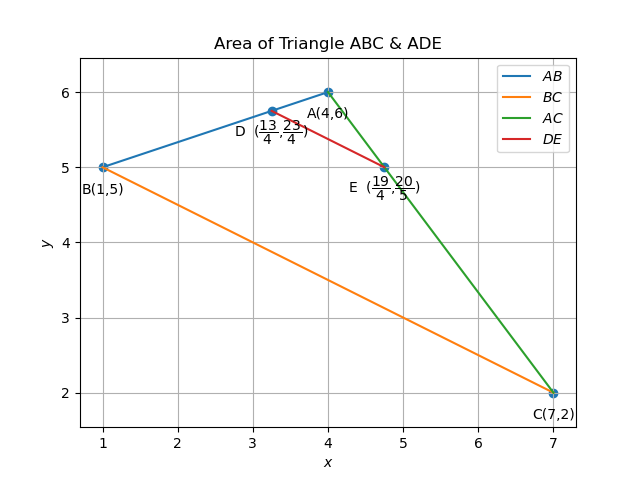
\includegraphics[width=\columnwidth]{chapters/10/7/4/6/figs/fig.png}
 \end{center}
\caption{}
\label{fig:chapters/10/7/4/6Fig1}
\end{figure}

    \item Draw a quadrilateral in the Cartesian plane, whose vertices are 
    \begin{align}
        \vec{A} = \myvec{-4\\5} \quad \vec{B} = \myvec{0\\7} \\
        \vec{C} = \myvec{5\\-5} \quad \vec{D} = \myvec{-4\\-2}
    \end{align}
    Also, find its area.
\label{chapters/11/10/1/1}
   \\ 
    \solution 
\iffalse
\documentclass[journal,12pt,twocolumn]{IEEEtran}
\usepackage{setspace}
\usepackage{gensymb}
\usepackage{xcolor}
\usepackage{caption}
\singlespacing
\usepackage{siunitx}
\usepackage[cmex10]{amsmath}
\usepackage{mathtools}
\usepackage{hyperref}
\usepackage{amsthm}
\usepackage{mathrsfs}
\usepackage{txfonts}
\usepackage{stfloats}
\usepackage{cite}
\usepackage{cases}
\usepackage{subfig}
\usepackage{longtable}
\usepackage{multirow}
\usepackage{enumitem}
\usepackage{mathtools}
\usepackage{listings}
\usepackage{tikz}
\usetikzlibrary{shapes,arrows,positioning}
\usepackage{circuitikz}
\let\vec\mathbf
\DeclareMathOperator*{\Res}{Res}
\renewcommand\thesection{\arabic{section}}
\renewcommand\thesubsection{\thesection.\arabic{subsection}}
\renewcommand\thesubsubsection{\thesubsection.\arabic{subsubsection}}

\renewcommand\thesectiondis{\arabic{section}}
\renewcommand\thesubsectiondis{\thesectiondis.\arabic{subsection}}
\renewcommand\thesubsubsectiondis{\thesubsectiondis.\arabic{subsubsection}}
\hyphenation{op-tical net-works semi-conduc-tor}

\lstset{
language=Python,
frame=single, 
breaklines=true,
columns=fullflexible
}
\begin{document}
\theoremstyle{definition}
\newtheorem{theorem}{Theorem}[section]
\newtheorem{problem}{Problem}
\newtheorem{proposition}{Proposition}[section]
\newtheorem{lemma}{Lemma}[section]
\newtheorem{corollary}[theorem]{Corollary}
\newtheorem{example}{Example}[section]
\newtheorem{definition}{Definition}[section]
\newcommand{\BEQA}{\begin{eqnarray}}
\newcommand{\EEQA}{\end{eqnarray}}
\newcommand{\define}{\stackrel{\triangle}{=}}
\newcommand{\myvec}[1]{\ensuremath{\begin{pmatrix}#1\end{pmatrix}}}
\newcommand{\mydet}[1]{\ensuremath{\begin{vmatrix}#1\end{vmatrix}}}

\bibliographystyle{IEEEtran}
\providecommand{\nCr}[2]{\,^{#1}C_{#2}} % nCr
\providecommand{\nPr}[2]{\,^{#1}P_{#2}} % nPr
\providecommand{\mbf}{\mathbf}
\providecommand{\pr}[1]{\ensuremath{\Pr\left(#1\right)}}
\providecommand{\qfunc}[1]{\ensuremath{Q\left(#1\right)}}
\providecommand{\sbrak}[1]{\ensuremath{{}\left[#1\right]}}
\providecommand{\lsbrak}[1]{\ensuremath{{}\left[#1\right.}}
\providecommand{\rsbrak}[1]{\ensuremath{{}\left.#1\right]}}
\providecommand{\brak}[1]{\ensuremath{\left(#1\right)}}
\providecommand{\lbrak}[1]{\ensuremath{\left(#1\right.}}
\providecommand{\rbrak}[1]{\ensuremath{\left.#1\right)}}
\providecommand{\cbrak}[1]{\ensuremath{\left\{#1\right\}}}
\providecommand{\lcbrak}[1]{\ensuremath{\left\{#1\right.}}
\providecommand{\rcbrak}[1]{\ensuremath{\left.#1\right\}}}
\theoremstyle{remark}
\newtheorem{rem}{Remark}
\newcommand{\sgn}{\mathop{\mathrm{sgn}}}
\newcommand{\rect}{\mathop{\mathrm{rect}}}
\newcommand{\sinc}{\mathop{\mathrm{sinc}}}
\providecommand{\abs}[1]{\left\vert#1\right\vert}
\providecommand{\res}[1]{\Res\displaylimits_{#1}} 
\providecommand{\norm}[1]{\left\Vert#1\right\Vert}
\providecommand{\mtx}[1]{\mathbf{#1}}
\providecommand{\mean}[1]{E\left[ #1 \right]}
\providecommand{\fourier}{\overset{\mathcal{F}}{ \rightleftharpoons}}
\providecommand{\ztrans}{\overset{\mathcal{Z}}{ \rightleftharpoons}}
\providecommand{\system}[1]{\overset{\mathcal{#1}}{ \longleftrightarrow}}
\newcommand{\solution}{\noindent \textbf{Solution: }}
\providecommand{\dec}[2]{\ensuremath{\overset{#1}{\underset{#2}{\gtrless}}}}
\let\StandardTheFigure\thefigure
\def\putbox#1#2#3{\makebox[0in][l]{\makebox[#1][l]{}\raisebox{\baselineskip}[0in][0in]{\raisebox{#2}[0in][0in]{#3}}}}
     \def\rightbox#1{\makebox[0in][r]{#1}}
     \def\centbox#1{\makebox[0in]{#1}}
     \def\topbox#1{\raisebox{-\baselineskip}[0in][0in]{#1}}
     \def\midbox#1{\raisebox{-0.5\baselineskip}[0in][0in]{#1}}

\vspace{3cm}
\title{Straight Lines Assignment}
\author{Gautam Singh}
\maketitle
\bigskip

\begin{abstract}
    This document contains the solution to Question 1 of Exercise 1 in Chapter
    10 of the class 11 NCERT textbook.
\end{abstract}

\begin{enumerate}
\fi
		The points are plotted in Fig. \ref{fig:11/10/1/1quad}. The plot is 
    generated using the Python code \texttt{codes/quad.py}.

    The area vector (denoted by $\vec{R_X}$ for region $X$) of the quadrilateral 
    is perpendicular to the plane of the quadrilateral and its orientation is 
    assumed to be in the positive $z$-direction here.
    \begin{align}
        &\vec{R_{ABCD}} = \vec{R_{ABC}} + \vec{R_{ACD}} \\
        &= \frac{1}{2}\brak{\brak{\vec{B}-\vec{A}}\times\brak{\vec{C}-\vec{A}} + 
        \brak{\vec{C}-\vec{A}}\times\brak{\vec{D}-\vec{A}}} \\
        &= \frac{1}{2}\brak{\brak{\vec{C}-\vec{A}}\times
        \brak{\vec{D}-\vec{A}+\vec{A}-\vec{B}}} \\
        &= \frac{1}{2}\brak{\brak{\vec{C}-\vec{A}}\times\brak{\vec{D}-\vec{B}}} \\
        \label{eq:11/10/1/1area-diag} 
    \end{align}
    Thus the area of quadrilateral ABCD is
    \begin{align}
        \textrm{ar}\brak{ABCD} &= \norm{\vec{R_{ABCD}}} \\
                               &= \frac{1}{2}\norm{\brak{\vec{C}-\vec{A}}\times\brak{\vec{D}-\vec{B}}} \\ 
                               &= \frac{1}{2}\mydet{9&-4\\-10&-9} \\
                               &= 60.5\ \textrm{sq. units.}
        \label{eq:11/10/1/1ans}
    \end{align}
    \begin{figure}[!htb]
        \centering
        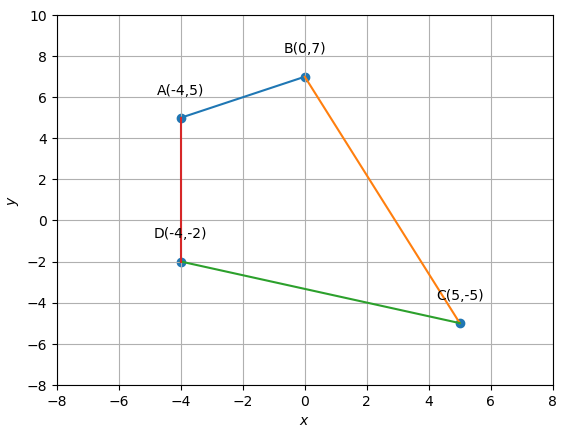
\includegraphics[width=\columnwidth]{chapters/11/10/1/1/figs/quad.png}
        \caption{Plot of quadrilateral $ABCD$}
        \label{fig:11/10/1/1quad}
    \end{figure}

\item Find the area of region bounded by the triangle whose
	vertices are $(1, 0), (2, 2) \text{ and } (3, 1)$. 
\item Find the area of region bounded by the triangle whose vertices
	are $(– 1, 0), (1, 3) \text{ and } (3, 2)$. 
\item Find the area of the $\triangle ABC$, coordinates of whose vertices are $\vec{A}(2, 0), \vec{B}(4, 5), \text{ and } \vec{C}(6, 3)$.

\end{enumerate}

